\section{Oscillatore Armonico Quantistico Unidimensionale}

	Il problema dell'oscillatore armonico è da sempre uno dei problemi più importanti della fisica. Come mai?
	\\
	\\
	Molti sistemi fisici possono essere ricondotti ad esso, quasi tutti in effetti. In cosa consiste il problema dell'oscillatore armonico nell'ambito della Meccanica Quantistica?

\begin{nb}
	Il problema dell'\textit{oscillatore armonico} nell'ambito della Meccanica Quantistica consiste nel risolvere il problema agli autovalori associato ad un Hamiltoniana con potenziale (energia potenziale) armonico.
\end{nb}

	Fino ad ora abbiamo trovato 3 diverse rappresentazioni, tutte equivalenti fra loro. Per capire quale convenga usare dobbiamo interrogarci sul tipo di richiesta che ci viene fatta. A domande fisiche diverse, corrispondono rappresentazioni differenti. Trattiamo allora, l'oscillatore armonico quantistico unidimensionale nelle tre, diverse, rappresentazioni.


\subsection{Rappresentazione Olomorfa}

	Come scriviamo le osservabili in questa rappresentazione?
	\\
	\\
	Ricordiamo che $\hat{a}$ ed $\hat{a}^{\dagger}$ non sono hermitiani, allora non è possibile associare loro direttamente un osservabile.

\begin{myapprf}
	Ricordiamo che: \textit{gli osservabili fisici devono essere associati ad operatori hermitiani (o autoaggiunti).}
	\\
	\\
	Infatti un operatore hermitiano (autoaggiunto) $\hat{O} = \hat{O}^{\dagger}$ garantisce proprietà fondamentali, tra cui:
\begin{itemize}
	\item \textit{Valori propri reali:}
	
		La condizione di hermitianità implica che tutti gli autovalori siano reali, e questi valori rappresentano i risultati possibili di una misura fisica.
		
	\item \textit{Autostati ortogonali:}
	
		Gli autostati di un operatore hermitiano formano una base ortonormale, ideale per la descrizione fisica di uno spazio di Hilbert.
\end{itemize}

	Al contrario gli operatori \textit{non} hermitiani:
	
\begin{itemize}
	\item Non hanno autovalori necessariamente reali.
	\item Non corrispondono direttamente ad una quantità misurabile fisicamente.
\end{itemize}
\end{myapprf}

	Allora come facciamo? possiamo associare un osservabile ad un operatore "composto" diciamo, definiamo infatti:
	
\begin{mydef}
	Definisco il nuovo \textbf{operatore numero} che ha il compito di contare lo stato, come:
\begin{align*}
	\hat{N} = \hat{a}^{\dagger}\hat{a}
\end{align*}
	che è \textit{hermitiano} e dunque a cui è possibile associarci un osservabile.
\end{mydef}

	dimostriamo quindi che effettivamente $\hat{N}$ è hermitiano:
	
\begin{myprf}
	$\hat{N}$ è hermitiano se:
\begin{align*}
	\hat{N} = \hat{N}^{\dagger}
\end{align*}
	allora:
\begin{align*}
	\hat{N}^{\dagger} = \qty(\hat{a}^{\dagger}\hat{a})^{\dagger}
\end{align*}	
	ricordiamo allora la proprietà dell'operazione di trasposta coniugata ovvero:
\begin{align*}
	\qty(\hat{A}\hat{B})^{\dagger} = \hat{B}^{\dagger}\hat{A}^{\dagger}
\end{align*}
	allora:
\begin{align*}
	\qty(\hat{a}^{\dagger}\hat{a})^{\dagger} = \hat{a}^{\dagger} \qty(\hat{a}^{\dagger})^{\dagger} = \hat{a}^{\dagger} \hat{a} = \hat{N}
\end{align*}
	abbiamo quindi dimostrato che effettivamente $\hat{N}$ è hermitiano.
\end{myprf}

	Questa rappresentazione è perfetta per trovare gli autostati $\hat{N}$. Esplicitiamo allora i termini ricordando che:
	
\begin{align*}
	\hat{a} = N \, \qty(\hat{p} - i\, m\omega \, \hat{x}) \qquad ; \qquad \hat{a}^{\dagger} = N \, \qty(\hat{p} + i\, m\omega \, \hat{x})
\end{align*}

	con $N$ costante che vale:
	
\begin{align*}
	N = \frac{1}{\sqrt{2m\omega \hbar}}
\end{align*}

	allora vale che sostituendo in $\hat{N}$, ottengo:
	
\begin{align*}
	\hat{N} = \hat{a}^{\dagger}\hat{a} & = \frac{1}{2m\omega \hbar} \, \qty\big(\hat{p} + im\omega \, \hat{x}) \,  \qty\big(\hat{p} - im\omega \, \hat{x}) = \frac{1}{2m\omega \hbar} \, \qty\big( \hat{p}^2 - im\omega \, \hat{p}\hat{x} + im\omega \, \hat{x}\hat{p} + m^2\omega^2 \, \hat{x}^2) \\
	& = \frac{1}{2m\omega \hbar} \, \qty\Big( \hat{p}^2  + im\omega \,\textcolor{blue}{\qty\big( \hat{x}\hat{p} - \hat{p}\hat{x})} + m^2\omega^2 \, \hat{x}^2) = \frac{1}{2m\omega \hbar} \, \qty\Big( \hat{p}^2  + im\omega \,\textcolor{blue}{\qty\big[ \hat{x}, \hat{p}]} + m^2\omega^2 \, \hat{x}^2)
\end{align*}
	
	ricordiamo ora che:
	
\begin{align*}
	\qty\big[\hat{x}, \hat{p}] = i\hbar \mathbb{I}
\end{align*}

	allora sostituisco:

\begin{align*}
	\hat{N} & = \frac{1}{2m\omega \hbar} \, \qty\Big( \hat{p}^2  + im\omega \,\textcolor{blue}{\qty(i\hbar \mathbb{I})} + m^2\omega^2 \, \hat{x}^2) = \frac{1}{2m\omega \hbar} \, \qty\Big( \hat{p}^2  - m\omega\hbar + m^2\omega^2 \, \hat{x}^2) \\
	& = \frac{1}{2m\omega \hbar} \, \qty\Big( \hat{p}^2 + m^2\omega^2 \, \hat{x}^2 - m\omega\hbar ) = \frac{1}{\hbar \omega} \, \qty(\frac{\hat{p}^2}{2m} + \frac{1}{2}m\omega^2 \, \hat{x}^2 - \frac{\omega\hbar}{2})  
\end{align*}

	porto allora fuori l'ultimo termine ed ottengo:
	
\begin{align*}
	\hat{N} = \frac{1}{\hbar \omega} \, \qty(\frac{\hat{p}^2}{2m} + \frac{1}{2}m\omega^2 \, \hat{x}^2) - \frac{1}{2}  
\end{align*}
		
	e riordino ottenendo:

\begin{nb}
\begin{align*}
	\frac{\hat{p}^2}{2m} + \frac{1}{2}m\omega^2 \, \hat{x}^2 = \hbar \omega \, \qty(\hat{N} + \frac{1}{2})
\end{align*}
\end{nb}
	
	da questa equazione definiamo uno dei \textit{più importanti} operatori di tutta la meccanica quantistica, guardando a sinistra allora:

\begin{mydef}
	Definiamo l'\textbf{operatore Hamiltoniano} $\hat{H}$ del sistema:
\begin{align*}
	\hat{H} = \frac{\hat{p}^2}{2m} + \frac{1}{2}m\omega^2 \, \hat{x}^2
\end{align*}
	esso è associato direttamente all'energia del sistema.
\end{mydef}
	
	Allora sicuramente, data la definizione, vale anche l'uguaglianza:
	
\begin{align*}
	\hat{H} = \hbar \omega \, \qty(\hat{N} + \frac{1}{2})
\end{align*}

	trovando allora gli autostati di questa equazione si trovano gli autostati di $\hat{H}$ per un oscillatore armonico unidimensionale. Quali sono gli autostati allora di $\hat{H}$? Sono quegli stati $v_N$ tali vale:
	
\begin{align*}
	\hat{H}v_N = \hbar \omega \, \qty(\hat{N} + \frac{1}{2}) \, v_N
\end{align*}

	allora sarà più semplice risolvere al suo posto:
	
\begin{align*}
	\hat{N} v_{N} = N v_N
\end{align*}
	
	questo lo si sa a posteriori, infatti gli autostati di $\hat{N}$ sono noti come stati di numero o \textbf{stati di Fock}, e formano una base completa per lo spazio degli stati dell'oscillatore armonico. Questi stati sono ortonormali e permettono di espandere qualsiasi stato del sistema, compresa l'Hamiltoniana. Questo significa che, una volta trovati gli autostati e gli autovalori di $\hat{N}$ si ottiene immediatamente lo spettro energetico dell'oscillatore armonico. Quindi procediamo con l'approccio tramite $\hat{N}$ che permette di evitare la risoluzione diretta dell'equazione differenziale dell'oscillatore armonico.

\subsubsection{Base e Normalizzazione:}

	Devo quindi risolvere:
	
\begin{align*}
	\hat{N} v_{N} = N v_N
\end{align*}
	
	allora:
	
\begin{align*}
	\hat{N} v_{N} = N v_N \, \Rightarrow \, \hat{a}^{\dagger}\hat{a} v_N = N v_N \, \Rightarrow \, z \, \dv{z}v_N(z) = N v_N(z)
\end{align*}
	
	allora risolvo l'equazione differenziale:
	
\begin{align*}
	z \, \dv{z}v_N(z) = N v_N(z) \, \Rightarrow \, \frac{\dd v_N}{v_N} = N \, \frac{\dd z}{z} \, \Rightarrow \, \log v_N = N \log z + C = \log z^N + C \, \Rightarrow \, v_N =  C_N \, z^N
\end{align*}

	abbiamo quindi ottenuto:
	
\begin{align*}
	v_N =  C_N \, z^N
\end{align*}

	il nostro spazio degli stati è uno spazio di funzioni olomorfe e normalizzabili. Le funzioni in questo spazio sono dunque analitiche espandibili in $z$. Ciò significa anche che $N$ deve essere intero, cioè $N = \{ 0, 1, 2, \ldots \}$. In questo senso $N$ è il primo operatore a cui corrisponde un'osservabile con spettro discreto in dimensione infinita.
	\\
	\\
	Essendo gli stati normalizzabili troviamone allora la norma partendo dalla definizione di prodotto scalare nella rappresentazione olomorfa:
	
\begin{align*}
	\braket{w}{v} = \int_{\mathbb{C}} \dd^2 z \, N \, e^{\, -z\overline{z}} \, w^*(\overline{z}) \, v(z)
\end{align*}

	sostituiamo:
	
\begin{itemize}
	\item $w = v_N = C_N \, z^N$
	\item $v = v_N = C_N \, z^N$
\end{itemize}

	allora:
	
\begin{align*}
	\braket{v_N}{v_N} = \int_{\mathbb{C}} \dd^2 z \, \gamma \, e^{\, - z \overline{z}} \, \overline{z}^{N} \, z^N
\end{align*}
	
	dove ho usato il fatto che $v_N = C_N \, z^N$ e ho usato il fatto che $\gamma$ è una costante che raccoglie il fattore $C_N$ più il fattore $N$ di normalizzazione che avevamo inserito nel prodotto scalare della rappresentazione olomorfa. Dunque:
	
\begin{align*}
	\braket{v_N}{v_N} = C^2_N \, \gamma' \int_{\mathbb{C}} \dd^2 z \, e^{\, -z \overline{z}} \, \overline{z}^N \, z^N
\end{align*}

	Passiamo ora in coordinate polari, con:
	
\begin{itemize}
	\item $z = r \, e^{ \, i \theta}$
	\item $\overline{z} = r \, e^{ \,- i\theta}$
\end{itemize}

\begin{align*}
	\braket{v_N}{v_N} = C^2_N \, \gamma' \int_0^{2\pi}\int_0^{\infty} \dd r \dd \theta \, r \, e^{\, -r^2} \, r^N e^{\, iN\theta} \, r^N e^{\, - iN\theta} = C_N^2 \, \gamma' \int_0^{2\pi}\int_0^{\infty} \dd r \dd \theta \, r \, e^{\, -r^2} \, r^{2N}
\end{align*}

	sia ora $\xi = r^2$, allora:
	
\begin{align*}
	\dd \xi = 2 r \, \dd r \, \Rightarrow \, \dd r = \frac{\dd \xi}{2 r }
\end{align*}
	
	e quindi:
	
\begin{align*}
	\braket{v_N}{v_N} = C_N^2 \, \gamma' \int_0^{2\pi}\int_0^{\infty} \dd r \dd \theta \, r \, e^{\, -r^2} \, r^{2N} &= \frac{1}{2} \, 2\pi \, C_N^2 \, \gamma' \int_0^{2\pi}\int_0^{\infty} \dd \xi \dd \theta  \, e^{\, -\xi} \, \xi^{N} \\
	&= \pi \, C_N^2 \, \gamma' \int_0^{\infty} \dd \xi \, e^{\, -\xi} \, \xi^{N}
\end{align*}

	quindi per ora abbiamo ottenuto:

\begin{nb}
\begin{align*}
	\braket{v_N}{v_N} = \pi \, C_N^2 \, \gamma' \textcolor{ForestGreen}{\int_0^{\infty} \dd \xi \, e^{\, -\xi} \, \xi^{N}}
\end{align*}
\end{nb}

	mi chiedo allora quanto valga il generale l'integrale:
	
\begin{align*}
	I(\alpha) = \int_0^{ \infty} e^{\, -\alpha \xi} \, \xi^N \, \dd \xi
\end{align*}

	il risultato è:
	
\begin{align*}
	I(\alpha) = \frac{N!}{\alpha^{N+1}}
\end{align*}

	come si trova? Vediamo un piccolo approfondimento:
	
\begin{myapprf}
	Per risolvere l'integrale cui sopra dobbiamo utilizzare un metodo chiamato: \textit{trucco di Feynman}.
	\\
	\\
	Prima di tutto sappiamo che possiamo calcolare velocemente:
\begin{align*}
	\int_0^{\infty} e^{\, -\alpha \xi} \dd \xi = \qty[-\frac{1}{\alpha} \, e^{\, -\alpha \xi}]^{\infty}_0
\end{align*}

	pensando appunto al risultato come alla funzione che derivata mi ridà l'integranda. Allora essendo l'integrale improprio ne faccio il limite:

\begin{align*}
	\int_0^{\infty} e^{\, -\alpha \xi} \dd \xi = \lim_{b \to \infty}\qty[-\frac{1}{\alpha} \, e^{\, -\alpha \xi}]^{b}_0 = \lim_{b\to \infty}\qty(-\frac{1}{\alpha} \, e^{\, -\alpha  b} + \frac{1}{\alpha})
\end{align*}

	allora essendo:
	
\begin{align*}
	\lim_{b\to \infty} \frac{1}{\alpha} \, e^{\, -\alpha  b} = 0
\end{align*}

	si ottiene:
	
\begin{align*}
	\int_0^{\infty} e^{\, -\alpha \xi} \dd \xi =\frac{1}{\alpha}
\end{align*}
	
	Allora il trucco è quello di derivare $N$-esimamente in $-\alpha$ sia a sinistra che a destra ed ottenere:
	
\begin{align*}
	\textcolor{orange}{- \pdv[N]{\alpha} \int_0^{\infty} e^{\, -\alpha \xi} \dd \xi} = \textcolor{blue}{ - \pdv[N]{\alpha}  \frac{1}{\alpha}}
\end{align*}

	posso scambiare integrale e derivata poiché l'integranda è infinitamente differenziale e perché l'integrazione converge, dunque:

\begin{align*}
	- \pdv[N]{\alpha} \int_0^{\infty} e^{\, -\alpha \xi} \dd \xi = - \int_0^{\infty} \pdv[N]{\alpha}  e^{\, -\alpha \xi} \dd \xi
\end{align*}
	
	quanto vale la derivata $N$-esima?
	
\begin{align*}
	\pdv[N]{\alpha}  e^{\, -\alpha \xi} = \qty(-\xi)^N  e^{\, -\alpha \xi}
\end{align*}

	allora:
	
\begin{align*}
	- \int_0^{\infty} \pdv[N]{\alpha}  e^{\, -\alpha \xi} \dd \xi =  - \int_0^{\infty} \qty(-\xi)^N  e^{\, -\alpha \xi}  \dd \xi
\end{align*}

	possiamo ora riscrivere:

\begin{align*}
	-\qty(-\xi)^N = (-1)^{N+1} \, \xi^N
\end{align*}
	
	posso riscrivere allora:

\begin{align*}
	- \int_0^{\infty} \qty(-\xi)^N  e^{\, -\alpha \xi}  \dd \xi = \int_0^{\infty}  (-1)^{N+1} \, \xi^N  e^{\, -\alpha \xi}  \dd \xi = \textcolor{orange}{  (-1)^{N+1} \int_0^{\infty} \xi^N  e^{\, -\alpha \xi}  \dd \xi}
\end{align*}
	
	pensando ora alla parte destra invece:
	
\begin{align*}
	- \pdv[N]{\alpha}  \frac{1}{\alpha} = - (-1)^N \, \frac{N!}{\alpha^{N+1}} =  \textcolor{blue}{ (-1)^{N+1} \, \frac{N!}{\alpha^{N+1}}}
\end{align*}

	dove tale valore della derivata si può ottenere tramite induzione. 
	\\
	\\
	Ora mettiamo tutto insieme:
	
\begin{align*}
	\textcolor{orange}{  (-1)^{N+1} \int_0^{\infty} \xi^N  e^{\, -\alpha \xi}  \dd \xi} = \textcolor{blue}{(-1)^{N+1} \, \frac{N!}{\alpha^{N+1}}}  
\end{align*}
	
	semplificando allora:
	
\begin{align*}
	 \textcolor{red}{ \int_0^{\infty} \xi^N  e^{\, -\alpha \xi}  \dd \xi} =  \frac{N!}{\alpha^{N+1}}
\end{align*}

	e allora: 
	
\begin{align*}
	\textcolor{red}{ I(\alpha)} = \frac{N!}{\alpha^{N+1}}
\end{align*}
\end{myapprf}

	allora da:

\begin{align*}
	\braket{v_N}{v_N} = \pi \, C_N^2 \, \gamma' \int_0^{\infty} \dd \xi \, e^{\, -\xi} \, \xi^{N} = \pi \, C_N^2 \, \gamma' \, I(\alpha = 1)
\end{align*}

	essendo che vale:
	
\begin{align*}
	I(\alpha) = \frac{N!}{\alpha^{N+1}} \, \Rightarrow \, I(\alpha = 1) = N!
\end{align*}

	pertanto la norma di $v_N$ è:

\begin{nb}
\begin{align*}
	\braket{v_N} = C_N^2 \pi \gamma' N!
\end{align*}
\end{nb}

	Per comodità non voglio tenere il fattore $\pi$, perciò scelgo di definire:
	
\begin{align*}
	\gamma' = \frac{1}{\pi}
\end{align*}

	allora scriviamo il prodotto scalare:

\begin{align*}
	\braket{w}{v} =  \int_{\mathbb{C}} \dd^2 z \, \gamma\, e^{\, -z\overline{z}} \, w^*(z) \, v(z) = \gamma \int_{\mathbb{C}} \dd^2 z \, e^{\, -z\overline{z}} \, w^*(z) \, v(z)
\end{align*}

	scrivendo: $\gamma = 1/\pi$, dunque:
	
\begin{align*}
	\braket{w}{v} = \frac{1}{\pi} \int_{\mathbb{C}} \dd^2 z \, e^{\, -z\overline{z}} \, w^*(z) \, v(z)
\end{align*}

	dunque avrei che che:

\begin{nb}
\begin{align*}
	\braket{v_N} = \frac{1}{\pi} \, \pi N! = N!
\end{align*}
\end{nb}

	ma voglio una normalizzazione ad $1$, quindi imponendo questa condizione trovo i coefficienti $C_N$, prima di tutto sappiamo:

\begin{align*}
	v_N = C_N \, z^N 
\end{align*}
	
	allora fisso:
	
\begin{align*}
	\braket{v_N} = 1 \, \Leftrightarrow \, \braket{C_N \, z^N }{C_N \, z^N } = 1 \, \Leftrightarrow \, C_N^2 \braket{z^N} = 1
\end{align*}

	notiamo però che, dalla definizione di prodotto scalare:
	
\begin{align*}
	\braket{z^N} = \frac{1}{\pi} \int_{\mathbb{C}} \dd^2z \, e^{\, -z\overline{z}} \overline{z}^N \, z^N
\end{align*}

	che allora è proprio:
	
\begin{align*}
	\frac{1}{\pi} \int_{\mathbb{C}} \dd^2z \, e^{\, -z\overline{z}} \overline{z}^N \, z^N = N!
\end{align*}

	e dunque possiamo dire che:
	
\begin{align*}
	C_N^2 \, N! = 1 \, \Rightarrow \, \textcolor{blue}{C_N} = \frac{1}{\sqrt{N!}}
\end{align*}

	e possiamo inoltre scrivere l'autostato come:

\begin{align*}
	v_N = \textcolor{blue}{C_N} \, z^N = \textcolor{blue}{\frac{\textcolor{black}{z^N}}{\sqrt{N!}}}
\end{align*}

	ne segue che abbiamo trovato che:
	
\begin{mydef}
	$\hat{N}$ è un operatore hermitiano con autovalori interi, la cui \textbf{base}, \textbf{di dimensione infinita}, è:
\begin{align*}
	\qty{\frac{z^N}{\sqrt{N!}}}
\end{align*}
\end{mydef}

\begin{myprop}
	La base di $\hat{N}$, è \textbf{ortonormale} ovvero tale che:
\begin{align*}
	\braket{v_N}{v_M} = \delta_{NM}
\end{align*}
\end{myprop}

\begin{myprf}
	Per dimostrarlo ci basta calcolare: $\braket{v_N}{v_M}$ esplicitamente, ovvero:

\begin{align*}
	\braket{v_N}{v_M} = \frac{1}{\pi} \int_{\mathbb{C}} \dd^2 z \, e^{\, -z\overline{z}} \, v^*_N(z)\, v_M(z) 
\end{align*}

\begin{itemize}
	\item $v^*_N(z) = C_N \, \overline{z}^N$
	\item $v_M(z) =  C_M  \, z^M$
\end{itemize}
	
\begin{align*}
	\braket{v_N}{v_M} = \textcolor{orange}{C_N} \, \textcolor{Magenta}{C_M} \, \frac{1}{\pi}\int_{\mathbb{C}} \dd^2 z \, e^{\, -z\overline{z} }\, \overline{z}^N \, z^M & = \textcolor{orange}{\frac{1}{\sqrt{N!}}} \, \textcolor{Magenta}{\frac{1}{\sqrt{M!}}} \, \frac{1}{\pi}\int_{\mathbb{C}} \dd^2 z \, e^{\, -z\overline{z} }\, \overline{z}^N \, z^M \\
	&= \frac{1}{\pi \, \sqrt{N! \, M!}}\int_{\mathbb{C}} \dd^2 z \, e^{\, -z\overline{z} }\, \overline{z}^N \, z^M 
\end{align*}

	passo in coordinate polari:
	
\begin{itemize}
	\item $z = r e^{ i\theta}$
	\item $\overline{z} = r e^{\,- i\theta}$
\end{itemize}

\begin{align*}
	\braket{v_N}{v_M}  = \frac{1}{\pi \, \sqrt{N! \, M!}}\int_{\mathbb{C}} \dd^2 z \, e^{\, -z\overline{z} }\, \overline{z}^N \, z^M & = \frac{1}{\pi \, \sqrt{N! \, M!}}\int_{0}^{2\pi} \int_0^{\, \infty} r \dd r \dd \theta \,e^{\, -r^2}\,  r^{N} e^{\, - iN\theta} \, r^{M}  e^{\,iM\theta} \\
	& = \frac{1}{\pi \, \sqrt{N! \, M!}}\int_{0}^{2\pi}e^{\,iM\theta - iN\theta }  \dd \theta \int_0^{\, \infty} \dd r \, r \, e^{\, -r^2}\,  r^{N+M} \\
	& = \frac{1}{\pi \, \sqrt{N! \, M!}} \textcolor{blue}{\int_{0}^{2\pi}e^{\,i\theta\, \qty(M-N) }  \dd \theta }\int_0^{\, \infty} \dd r \, r \, e^{\, -r^2}\,  r^{N+M} 
\end{align*}

	fissiamo:
	
\begin{align*}
	n = M -N 
\end{align*}

	allora:

\begin{align*}
	\int_{0}^{2\pi}e^{\,i\theta\, \qty(M-N) }  \dd \theta  = \int_{0}^{2\pi}e^{\,i\theta n}  \dd \theta = \textcolor{blue}{2\pi \, \delta_{n0} }= \begin{cases}
		& 2\pi \quad \text{se $n =0 \, \Rightarrow \, $ se $M = N$} \\
		& 0 \quad \text{se $n \neq 0 \, \Rightarrow \, $ se $M \neq N$}
	\end{cases}
\end{align*}

	questo implica che o $M = N$, oppure $\braket{v_N}{v_M}$ è nullo. Allora in parte è soddisfatto ciò di cui abbiamo bisogno, non serve dimostrare esplicitamente che se $M = N$ allora $\braket{v_N}{v_M} = \braket{v_N} = 1$ poiché lo abbiamo già fatto nei paragrafi precedenti. Possiamo velocemente concludere allora che:
	
\begin{align*}
	\braket{v_N}{v_M} = \delta_{NM}
\end{align*}
	
	cioè che:
	
\begin{align*}
	\qty{\frac{z^N}{\sqrt{N!}}}
\end{align*}

	è una \textit{base ortonormale}.
	
\end{myprf}

\subsubsection{Livelli Energetici:}

	Abbiamo quindi affrontato la questione della normalizzazione e della base, torniamo ora all'equazione di partenza:
	
\begin{align*}
	\hat{N} v_N = N v_N
\end{align*}

	ci chiediamo prima di tutto se $\hat{N}$ ed $\hat{H} $ commutino, ci aspettiamo di si:

\begin{align*}
	\qty[\hat{N}, \hat{H}] = \qty[\hat{N}, \, \hbar \omega \qty(\hat{N} + \frac{1}{2})] & = \hbar \omega \, \hat{N} \qty(\hat{N} + \frac{1}{2} ) - \hbar \omega \, \qty(\hat{N} + \frac{1}{2} ) \hat{N} \\
	& = \hbar \omega \, \qty(  \hat{N} \qty(\hat{N} + \frac{1}{2} ) - \qty(\hat{N} + \frac{1}{2} ) \hat{N}) \\
	& = \hbar \omega \, \qty( \hat{N}^2 + \frac{\hat{N}}{2} - \hat{N}^2 -\frac{\hat{N}}{2} ) = 0
\end{align*}

	chiaramente allora, poiché: 

\begin{align*}
	\qty[\hat{N}, \hat{H}] = 0
\end{align*}

	allora ho che $\hat{N}$ ed $\hat{H}$ commutano. Questo significa che gli autostati di $\hat{H}$ sono anche autostati di $\hat{N}$. Faccio quindi agire $\hat{H}$ su di uno stato generico $v_N$. L'obiettivo ora è risolvere l'equazione agli autovalori:
	
\begin{align*}
	\hat{H} \ket{E} = E \ket{E}
\end{align*}

	e trovare gli autovalori $E$, ovvero sia l'energia del sistema. Fissiamo quindi:
	
\begin{align*}
	v_N = \ket{E}
\end{align*}
 
	Vediamo:
	
\begin{align*}
	\hat{H} = \hbar \omega \, \qty(\hat{N} + \frac{1}{2}) \, \Rightarrow \, \hat{H} v_N = \hbar \omega \, \qty(\hat{N} + \frac{1}{2})v_N 
\end{align*}

	so però che:
	
\begin{align*}
	\hat{N} v_N = Nv_N
\end{align*}

	dunque possiamo sostituire prima con:

\begin{align*}
	\hat{H} v_N = \hbar \omega \, \qty(N + \frac{1}{2})v_N 
\end{align*}

	allora, in conclusione possiamo dire:
	
\begin{mydef}
	I \textbf{livelli energetici} dell'oscillatore armonico quantistico unidimensionali sono dati da:
\begin{align*}
	E_N = \hbar \omega \, \qty(N + \frac{1}{2}) \quad ; \quad N = 0, 1, 2, 3, \ldots
\end{align*}
\end{mydef}

	dunque se nella teoria classic a lo stato ad energia più bassa per un oscillatore armonico è quando è fermo, nella teoria quantistica si definisce:
	
\begin{mydef}
	Definiamo lo \textbf{stato fondamentale} (o \textit{stato di vuoto}, \textit{ground state}) come $E_N$ per $N = 0$:
\begin{align*}
	E_0 = \frac{1}{2}\, \hbar \omega
\end{align*}
\end{mydef}

	allora a differenza della teoria classica, il ground state è \textit{non} nullo. Come ci aspettavamo inoltre \textit{l'energia è quantizzata}, nel senso che sono permessi solo determinati livelli di energia.
	\\
	\\ 
	Introduciamo ora nuovi concetti, \textit{come passo da un livello energetico all'altro?}

\begin{mydef}
	Data un qualsiasi funzione olomorfa, essa può essere scritta come:
\begin{align*}
	v(z) = \sum_{n=0}^{\infty} a_n \, \frac{z^n}{\sqrt{n!}}
\end{align*}
\end{mydef}
	
	si noti che uno stato è una funzione olomorfa mentre non tutte le funzioni olomorfe sono degli stati. Infatti affinché valga che tutte le funzioni olomorfe sia anche degli stati allora devono essere \textit{normalizzabili}. Si definisce:
	
\begin{mydef}
	Una \textit{funzione olomorfa normalizzabile}, ovvero sia \textit{uno stato}, vive nello \textbf{spazio delle successioni di numeri complessi a quadrato sommabile} $\textit{l}_2$, definito come:
\begin{align*}
	\textit{l}_2 = \qty{a_n \,\,\, \text{t.c} \,\,\, a_n \in \mathbb{C}  \,\, \text{e} \,\, \sum_{n=0}^{\infty} |a_n|^2 < \infty}
\end{align*}
\end{mydef}

	Abbiamo inoltre detto, nei paragrafi precedenti, che gli stati possiamo rappresentarli come:
	
\begin{align*}
	\qty{\frac{z^n}{\sqrt{n!}}} = \qty{\frac{z^0}{\sqrt{0!}}, \frac{z^1}{\sqrt{1!}}, \frac{z^2}{\sqrt{2!}}, \ldots  } = \qty{1, z, \frac{z^2}{\sqrt{2}}, \frac{z^3}{\sqrt{6}}, \ldots} \, \equiv \,  \qty\Big{\ket{0}, \ket{1}, \ket{2}, \ldots}
\end{align*}

	ovvero sia vogliamo:
	
\begin{nb}
	D'ora in poi rinominiamo lo stato con il valore dell'esponente dello stato stesso.
\end{nb}

	In questo modo possiamo riscrivere:
	
\begin{align*}
	\ket{n} = \frac{z^n}{\sqrt{n!}} = \frac{z^n}{\sqrt{n!}}  \cdot 1 = \frac{z^n}{\sqrt{n!}}  \, \ket{0}  
\end{align*}

	ricordo che:
	
\begin{align*}
	\hat{a}^{\dagger}v = z v
\end{align*}

	allora:
	
\begin{align*}
	\qty(\hat{a}^{\dagger})^n v = z^n v
\end{align*}

	e quindi possiamo scrivere:
	
\begin{align*}
	\qty(\hat{a}^{\dagger})^n \ket{0} = z^n \ket{0}
\end{align*}
	
	e allora:
	
\begin{align*}
	\ket{n} = \frac{z^n}{\sqrt{n!}}  \ket{0}   = \frac{\qty(\hat{a}^{\dagger})^n}{\sqrt{n!}}  \ket{0}  
\end{align*}

	questo espressione è fondamentale. Infatti vale che allora:
	
\begin{mydef}
	Definito il \textit{ground state}, \textbf{tutti gli altri autostati sono determinati} da:
\begin{align*}
	\ket{n} = \frac{\qty(\hat{a}^{\dagger})^n}{\sqrt{n!}} \ket{0}  
\end{align*}
\end{mydef}

	Perciò prendiamo uno \textit{stato generico} $\ket{v}$ allora si scrive che:
	
\begin{align*}
	\ket{v} = \sum a_n \ket{n} = \sum a_n \, \frac{\qty(\hat{a}^{\dagger})^n}{\sqrt{n!}} \ket{0}  
\end{align*}

	mi chiedo allora come agiscano gli operatori $\hat{a}^{\dagger}$ e $\hat{a}$ sugli stati. Vediamo, se facciamo:
	
\begin{align*}
	\hat{a}^{\dagger}\qty(\frac{z^n}{\sqrt{n!}}) = z \,\frac{z^n}{\sqrt{n!}} = \frac{z^{n+1}}{\sqrt{n!}} 
\end{align*}

	noto che posso riscrivere:
	
\begin{align*}
	\sqrt{n!}= \frac{\sqrt{n+1}}{\sqrt{\qty(n+1)!}}
\end{align*}

	allora posso sostituire:

\begin{align*}
	\hat{a}^{\dagger}\qty(\frac{z^n}{\sqrt{n!}}) = \frac{z^{n+1}}{\sqrt{n!}} = \sqrt{n+1} \, \textcolor{cyan}{ \frac{z^{n+1}}{\sqrt{\qty(n+1)!}} } = \sqrt{n+1} \, \, \textcolor{cyan}{\ket{n+1}}
\end{align*}

	perciò possiamo dire che:
	
\begin{mydef}
	Allora $\hat{a}^{\dagger}$ viene chiamato \textbf{operatore di salita} o \textbf{di creazione}, in quanto \textbf{crea} un quanto di energia, infatti la sua applicazione ad uno stato $\ket{n}$ da come risultato uno stato $\ket{n+1}$, ovvero:

\begin{align*}
	\hat{a}^{\dagger} \ket{n}= \sqrt{n+1} \ket{n+1}
\end{align*}
\end{mydef}

	In maniera del tutto analoga vediamo come agisce l'operatore $\hat{a}$ sullo stato generico $\ket{v}$:

\begin{align*}
	\hat{a} \qty(\frac{z^n}{\sqrt{n!}}) = \dv{z}\qty(\frac{z^n}{\sqrt{n!}}) = n \, \frac{z^{n-1}}{\sqrt{n!}} = n \, \frac{z^{n-1}}{\sqrt{n}\, \sqrt{\qty(n-1)!}}  = \sqrt{n} \, \frac{z^{n-1}}{\sqrt{\qty(n-1)!}} = \sqrt{n} \, \ket{n-1}
\end{align*}

	allora possiamo dire che:

\begin{mydef}
	Allora $\hat{a}$ viene chiamato \textbf{operatore di discesa} o \textbf{di distruzione}, in quanto \textbf{distrugge} un quanto di energia, infatti la sua applicazione ad uno stato $\ket{n}$ da come risultato uno stato $\ket{n-1}$, ovvero:

\begin{align*}
	\hat{a} \ket{n}= \sqrt{n} \ket{n-1}
\end{align*}
\end{mydef}

\begin{nb}
	In particolare, lo stato vuoto si dice che è "ammazzato" dall'\textit{operatore di discesa}, ovvero vale che:
	
\begin{align*}
	\hat{a} \ket{0} = 0
\end{align*}
\end{nb}

	In sostanza dunque, abbiamo trovato un modo per passare da un livello energetico ad un altro nell'oscillatore armonico.
	
\subsubsection{Il potenziale armonico quantistico:}

	Si ricorda velocemente che, l'Hamiltoniana del sistema è:
	
\begin{align*}
	\hat{H} = \frac{\hat{p}^2}{2m} + \frac{1}{2}m\omega^2x^2
\end{align*}

	ricordiamo inoltre da \textit{meccanica analitica}:
	
\begin{align*}
	\hat{H} = \hat{T} + \hat{V}
\end{align*}

	allora diciamo che:
	
\begin{mydef}
	Il \textbf{potenziale armonico quantistico} è definito come:
\begin{align*}
	V(x) = \frac{1}{2}m\omega^2x^2
\end{align*}
\end{mydef}
	
	vediamo dunque un grafico. 
	
\subsubsection{Grafico del potenziale armonico quantistico:}

%%%%%%%
\vspace{1em}
%%%%%%%
\begin{minipage}{0.45\textwidth}
	 Il grafico a destra rappresenta il potenziale armonico quantistico unidimensionale, in cui è evidenziato come l'energia sia quantizzata. La curva blu rappresenta il potenziale armonico che vale:
	 
\begin{align*}
	V(x) = \frac{1}{2} m\omega^2x^2
\end{align*}

	Ossia l'energia potenziale di un oscillatore armonico classico. 
	
 \end{minipage}
\hfill
\begin{minipage}{0.4\textwidth}
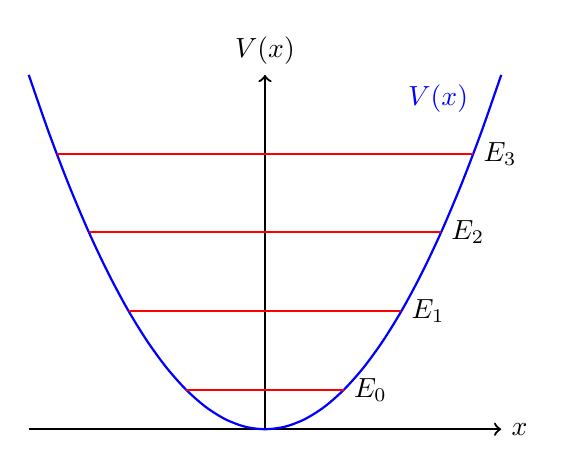
\begin{tikzpicture}
    % Assi cartesiani
    \draw[thick,->] (-3,0) -- (3,0) node[right] {$x$};
    \draw[thick,->] (0,0) -- (0,4.5) node[above] {$V(x)$};

    % Potenziale armonico
    \draw[domain=-3:3,smooth,variable=\x,thick,blue] plot ({\x},{0.5*\x*\x});

    % Livelli energetici
    \foreach \n in {0,1,2,3} {
        \draw[thick,red] (-{sqrt(2*\n+1)}, {0.5+\n}) -- ({sqrt(2*\n+1)}, {0.5+\n})
        node[right, black] {$E_{\n}$};
    }
    
    % Label del potenziale
    \node[blue] at (2.2,4.2) {$V(x)$};

\end{tikzpicture}

\end{minipage}
%%%%%%%
\vspace{1em}
%%%%%%%

	Le linee rosse orizzontali corrispondono invece ai livelli energetici permessi nella meccanica quantistica, dati dalla relazione:
	
\begin{align*}
	E_n = \hbar \omega \, \qty( n + \frac{1}{2}) \quad n = 0, 1, 2, \ldots
\end{align*}
	
	Fisicamente ciò implica che, diversamente dall'oscillatore classico che può assumere qualunque valore di energia, l'oscillatore quantistico può assumere esclusivamente energie discrete. Inoltre, anche nello stato fondamentale (il più basso, $E_0$), il sistema possiede un'energia diversa da zero, detta energia di ground state.

\subsubsection{Relazioni tra gli operatori numero e l'Hamiltoniana:}
	
	Esistono alcune relazioni tra i due operati $\hat{N}$ ed $\hat{H}$:
	
\vspace{1em}
\begin{minipage}{0.7\textwidth}
\begin{itemize}
	\item $\qty[\hat{H}, \hat{a}]  = - \hbar \omega \, \hat{a}$
	\item $\qty[\hat{H}, \hat{a}^{\dagger}]  = \hbar \omega \, \hat{a}^{\dagger}$
\end{itemize}
\end{minipage}
\hfill
\begin{minipage}{0.3\textwidth}
\begin{itemize}
	\item $\qty[\hat{N}, \hat{a}]  = - \hat{a}$
	\item $\qty[\hat{N}, \hat{a}^{\dagger}]  = \hat{a}^{\dagger}$
\end{itemize}
\end{minipage}
\vspace{1em}

	Con gli \textit{operatori di creazione} e \textit{di distruzione} che, ricordiamo, soddisfano le regole di commutazione:
	
\begin{align*}
	\qty[\hat{a}_i, \hat{a}_j] = 0 \quad ; \quad \qty[\hat{a}^{\dagger}_i, \hat{a}^{\dagger}_j] = 0 \quad ; \quad \qty[\hat{a}_i, \hat{a}^{\dagger}_j] = \delta_{ij}
\end{align*}
	
	Le relazioni di commutazione dell'\textit{operatore numero} con i due operatori permettono di definirne a priori la natura e trovare gli autostati dell'\textit{operatore numero}. Si ha a priori infatti che:

\begin{align*}
	& \hat{N}\hat{a}^{\dagger} \ket{n} = \qty(\qty[\hat{N}, \hat{a}^{\dagger}] + \hat{a}^{\dagger}\hat{N}) \ket{n} \\
	& \hat{N} \hat{a} \ket{n} = \qty(\qty[\hat{N}, \hat{a}] + \hat{a}\hat{N}) \ket{n}
\end{align*}

	tale scrittura deriva dal fatto che:
	
\begin{align*}
	&\qty[\hat{N}, \hat{a}^{\dagger}] = \hat{N}\hat{a}^{\dagger} - \hat{a}^{\dagger} \hat{N} \\
	& \qty[\hat{N}, \hat{a}] = \hat{N}\hat{a} - \hat{a}\hat{N} 
\end{align*}

	per definizione di commutatore. Inoltre essendo che:

\begin{align*}
	&\qty[\hat{N}, \hat{a}^{\dagger}] = \hat{a}^{\dagger} \\
	& \qty[\hat{N}, \hat{a}] =  - \hat{a}
\end{align*}

	posso sostituire ed ottenere:

\begin{align*}
	& \hat{N}\hat{a}^{\dagger} \ket{n} = \qty(\qty[\hat{N}, \hat{a}^{\dagger}] + \hat{a}^{\dagger}\hat{N}) \ket{n} =  \qty( \hat{a}^{\dagger} + \hat{a}^{\dagger}\hat{N}) \ket{n} = \hat{a}^{\dagger} \ket{n} + \hat{a}^{\dagger} \hat{N} \ket{n}\\
	& \hat{N} \hat{a} \ket{n} = \qty(\qty[\hat{N}, \hat{a}] + \hat{a}\hat{N}) \ket{n} =  \qty( - \hat{a} + \hat{a}\hat{N}) \ket{n} = - \hat{a} \ket{n} + \hat{a}\hat{N} \ket{n}
\end{align*}
	
	e gli autostati degli \textit{operatori di creazione} e \textit{distruzione} saranno proporzionali agli autostati: $\ket{n \pm 1}$ tramite i fattori di proporzionalità $c$ e $c'$:
	
\begin{align*}
	& \hat{a} \ket{n} = c \ket{n-1} \\
	& \hat{a}^{\dagger} \ket{n} = c' \ket{n+1}
\end{align*}
	
	per determinare i due fattori osserviamo che il valore di aspettazione dell'operatore numero sullo stato $\ket{n}$ è:
	
\begin{align*}
	n = \mel{n}{\hat{N}}{n} = \mel{n}{\hat{a}^{\dagger}\hat{a}}{n} = |c|^2 \geq 0
\end{align*} 

	da cui scopriamo che $n$ è un numero positivo. In modo analogo, si ha che:
	
\begin{align*}
	n = \mel{n}{\hat{a}^{\dagger}\hat{a}}{n} = \mel{n}{\hat{a}^{\dagger}\hat{a} -1 }{n} = \mel{n}{\hat{a}^{\dagger}\hat{a}}{n} - 1 = |c'|^2 -1
\end{align*}

	da cui si ottiene immediatamente che:
	
\begin{align*}
	& c = \sqrt{n}\\
	& c' = \sqrt{n+1}
\end{align*}

	poiché $n$ è un numero positivo e poiché l'azione degli operatori di creazione e distruzione aumentano o diminuiscono il valore di $n$ di un'unità, possiamo concludere che $n$ è un intero positivo e quindi: $n \in \mathbb{N}$.
	
\subsection{Rappresentazione di Schrodinger}

	Come avevamo già detto, diverse rappresentazioni, per diversi scopi. Utilizzeremo la rappresentazione di Schrodinger, nella descrizione dell'oscillatore armonico, per descrivere la probabilità che la particella si trovi nella posizione $x$, dato lo stato di energia più basso dell'oscillatore armonico. Questo concetto di probabilità è molto importante come già abbiamo visto nei capitoli precedenti.
	\\
	\\
	Partiamo dunque dalla rappresentazione di Schrodinger di $\hat{a}$ ed $\hat{a}^{\dagger}$ per vedere cosa succede al ground state $\ket{0}$. Se applichiamo l'operatore di discese al ground state otteniamo:
	
\begin{align*}
	\hat{a}\ket{0} = 0
\end{align*}

	Possiamo sostituire $\hat{a}$ con la sua definizione:
	
\begin{align*}
	\hat{a} = N \, \qty\big(\hat{p} - im\omega \, \hat{x}) \quad ; \quad N = \frac{1}{\sqrt{2m\hbar \omega}}
\end{align*}

	allora:

\begin{align*}
	\hat{a}\ket{0} =  \frac{1}{\sqrt{2m\hbar \omega}} \, \qty\big(\hat{p} - im\omega \, \hat{x}) \ket{0} = 0
\end{align*}

	dunque:

\begin{align*}
	\frac{1}{\sqrt{2m\hbar \omega}} \, \qty\big(\hat{p} - im\omega \, \hat{x}) \ket{0} = \frac{1}{\sqrt{2m\hbar \omega}} \, \qty\Big(\hat{p} \ket{0} - im\omega \, \hat{x} \ket{0}) 
\end{align*}

	dove allora:
	
\begin{align*}
	\hat{p}\ket{0} = - i \hbar \pdv{x} \ket{0} \qquad ; \qquad \hat{x}\ket{0} = x \ket{0} 
\end{align*}

	quindi:

\begin{align*}
	\frac{1}{\sqrt{2m\hbar \omega}} \, \qty\Big(\hat{p} \ket{0} - im\omega \, \hat{x} \ket{0})  = \frac{1}{\sqrt{2m\hbar \omega}} \, \qty( - i \hbar \pdv{x} - im\omega x) \ket{0} = 0 
\end{align*}

	come facciamo però a capire come appare lo stato $\ket{0}$ nella rappresentazione spaziale?
	\\
	\\
	Infatti $\ket{0}$ è uno stato astratto che vive nello spazio di Hilbert. Questo stato è rappresentato da un vettore astratto nello spazio degli stati quantistici. Non si tratta esplicitamente di una funzione in $x$, ma è solo un simbolo matematico che indica il ground state (stato fondamentale) del sistema. Allora per "vedere" come appare lo stato $\ket{0}$ nella rappresentazione spaziale, occorre proiettarlo su una base di autostati dell’operatore posizione $\hat{x}$. Questa base è formata dagli stati $\ket{x}$, che rappresentano lo stato in cui la particella è localizzata precisamente in un punto $x$, diciamo allora che:
	
\begin{align*}
	\psi_0(x) = \braket{x}{0}
\end{align*}

	Dunque, la \textit{funzione d'onda} $\psi_0(x)$ è il prodotto scalare tra lo stato astratto $\ket{0}$ e l'autostato $\ket{x}$ e ne segue dunque che: $\psi_0(x)$ è quindi \textit{la rappresentazione in coordinate spaziali dello stato astratto $\ket{0}$}. Bene, allora vale sicuramente che possiamo proiettare la quantità precedente, ovvero:

\begin{align*}
	 \frac{1}{\sqrt{2m\hbar \omega}} \, \qty( - i \hbar \pdv{x} - im\omega x) \ket{0} \, &\Rightarrow \, \frac{1}{\sqrt{2m\hbar \omega}} \, \qty( - i \hbar \pdv{x} - im\omega x) \textcolor{blue}{\braket{x}{0}} = 0 \\
	 & \Rightarrow \, \frac{1}{\sqrt{2m\hbar \omega}} \, \qty( - i \hbar \pdv{x} - im\omega x) \textcolor{blue}{\psi_0(x)} = 0
\end{align*}

	cerchiamo dunque la soluzione per $\psi_0(x)$, ovvero proseguiamo facendo:
	
\begin{align*}
	\frac{1}{\sqrt{2m\hbar \omega}} \, \qty( - i \hbar \pdv{x} - im\omega x) \psi_0(x) = 0 \, &\Leftrightarrow \,  \qty( - i \hbar \pdv{x} - im\omega x) \psi_0(x) = 0 \\
	& \Leftrightarrow \,  - i \hbar \pdv{x} \, \psi_0(x) - im\omega x  \psi_0(x) = 0 
\end{align*}

	allora:
	
\begin{align*}
	- i \hbar \pdv{x} \, \psi_0(x) = im\omega x  \psi_0(x) \, \Rightarrow \, \pdv{x}  \psi_0(x) = - \, \frac{m\omega }{\hbar} \, x \, \psi_0(x)
\end{align*}

	allora faccio le seguenti sostituzioni:
	
\begin{align*}
	\textcolor{orange}{\frac{m\omega}{\hbar}} = \frac{1}{\lambda^2} \qquad ; \qquad \textcolor{cyan}{\frac{x}{\lambda}} = \xi
\end{align*}

	allora:
	
\begin{align*}
	\pdv{x} \psi_0(x) = - \, \frac{m\omega }{\hbar} \, x \, \psi_0(x) \, \Rightarrow \, \pdv{x} \psi_0(x) = - \, \textcolor{orange}{\frac{1}{\lambda^2}} \, x \, \psi_0(x)
\end{align*}

	quindi:

\begin{align*}
	\pdv{x} \psi_0(x) = - \, \frac{x}{\lambda^2}  \, \psi_0(x)
\end{align*}

	allora essendo:
	
\begin{align*}
	\frac{x}{\lambda} = \xi \, \Rightarrow \, \frac{\dd x}{ \lambda} = \dd \xi \, \Rightarrow \, \dd x = \lambda \, \dd \xi
\end{align*}

	allora possiamo scrivere:
	
\begin{align*}
	\pdv{x} = \frac{\dd \xi}{\dd x} \pdv{\xi} = \frac{1}{\lambda} \, \pdv{\xi}
\end{align*}

	allora possiamo scrivere:
	
\begin{align*}
	\pdv{\xi} \psi_0(\xi) = - \textcolor{cyan}{{\xi}} \psi_0(\xi)
\end{align*}

	allora risolvo l'equazione differenziale:

\begin{align*}
	\pdv{\xi} \psi_0(\xi) = - \xi \psi_0(\xi) \, \Rightarrow \, \frac{\dd \psi_0(\xi)}{ \dd \xi} = - \xi \psi_0(\xi) \, \Rightarrow \, \frac{\dd \psi_0(\xi)}{\psi_0(\xi) } = - \xi \, \dd \xi \, \Rightarrow \, \log \psi_0(\xi) = - \frac{\xi^2}{2} + N
\end{align*}

	allora elevando tutto:

\begin{align*}
	\log \psi_0(\xi) = - \frac{\xi^2}{2} + N \, \Rightarrow \, \psi_0(\xi) = N \, e^{\, - \xi^2/2}
\end{align*}

	perciò scrivendo di nuovo:
	
\begin{align*}
	\frac{m\omega}{\hbar} = \frac{1}{\lambda^2} \qquad ; \qquad \frac{x}{\lambda} = \xi
\end{align*}

	si ottiene:

\begin{nb}
\begin{align*}
	\psi_0(x) = N' \, e^{\, - m\omega x^2/2\hbar}
\end{align*}
\end{nb}

	Possiamo allora dire che, quando mi trovo nello stato $\ket{0}$, la particella è sparpagliata attorno a $0$ con una gaussiana di larghezza $\lambda$. Perciò possiamo dire piuttosto che il ground state è \textit{uno stato di minima indeterminazione}. 
	\\
	\\
	Mi interessa allora capire quanto valga $N'$. Esso si può determinare normalizzando $\psi_0(x)$ ad $1$:
	
\begin{align*}
	|N'|^2 \int_{-\infty}^{\, + \infty} e^{\, - m\omega x^2/\hbar} \, \dd x = 1
\end{align*}

	dunque sapendo anche dai paragrafi precedenti che:
	
\begin{align*}
	\int_{-\infty}^{\, + \infty} e^{\, - \alpha x^2} \, \dd x = \sqrt{\frac{\pi}{\alpha}}
\end{align*}

	allora:
	
\begin{align*}
	|N'|^2 \, \sqrt{\frac{\pi \hbar}{m\omega}} = 1 \, \Rightarrow \, N' = \qty(\frac{m\omega}{\pi \hbar})^{1/4}
\end{align*}

	allora sostituendo:

\begin{nb}
\begin{align*}
	\psi_0(x) = \qty(\frac{m\omega}{\pi \hbar})^{1/4} \, e^{\, - m\omega x^2/2\hbar}
\end{align*}
\end{nb}

	si può anche fare lo stesso discorso nella rappresentazione degli impulsi, ma troveremmo lo stesso identico risultato.
	\\
	\\
	Continuiamo ora con lo stato $\ket{1}$. Per definizione si ha che:
	
\begin{align*}
	\psi_1(x) = \braket{x}{1}
\end{align*}

	e come lo definiamo $\ket{1}$? Possiamo definirlo con l'operatore di salita nel seguente modo:
	
\begin{align*}
	\hat{a}^{\dagger} \ket{0} = \ket{1}
\end{align*}

	allora scriviamo l'operatore di salita come:
	
\begin{align*}
	\hat{a}^{\dagger} = \frac{1}{\sqrt{2m\omega \hbar}} \, \qty\big(\hat{p} + im\omega \, \hat{x}) = \frac{1}{\sqrt{2m\omega \hbar}} \, \qty(- i \hbar \, \pdv{x} + im\omega \, x) 
\end{align*}

	allora sostituendo i parametri per la rappresentazione di Schrodinger 
	
\begin{align*}
	\frac{m\omega}{\hbar} = \frac{1}{\lambda^2} \qquad ; \qquad \frac{x}{\lambda} = \xi
\end{align*}

	allora:
	
\begin{align*}
	\frac{1}{\sqrt{2m\omega \hbar}} \, \qty(- i \hbar \, \pdv{x} + im\omega \, x) = \frac{\lambda}{\sqrt{2} \, \hbar} \, i \, \hbar \,  \qty(-  \, \pdv{x} +  \, \frac{x}{\lambda^2}) &= \frac{\lambda}{\sqrt{2}} \, i \,  \qty(-  \, \frac{1}{\lambda} \pdv{\xi} +  \, \frac{\xi}{\lambda})  \\
	& = \frac{i}{\sqrt{2}}\, \lambda \,  \qty(-  \, \frac{1}{\lambda} \pdv{\xi} +  \frac{\xi}{\lambda}) \\
	& =  \frac{i}{\sqrt{2}} \,  \qty(-  \,\pdv{\xi} +  \xi) \\
	& =  - \, \frac{i}{\sqrt{2}} \,  \qty\Big( \partial_{\xi} - \xi)
\end{align*}

	abbiamo quindi ottenuto:
	
\begin{align*}
	\hat{a}^{\dagger} = - \, \frac{i}{\sqrt{2}} \,  \qty\Big( \partial_{\xi} - \xi)
\end{align*}

	torniamo allora la definizione dello stato $\ket{1}$, vale allora:
	
\begin{align*}
	\ket{1} = \hat{a}^{\dagger} \ket{0} 
\end{align*}

	proiettando ora su $\ket{\xi}$
otteniamo:

\begin{align*}
	\braket{\xi}{1} = \hat{a}^{\dagger} \braket{\xi}{0} \, \Rightarrow \, \psi_1(\xi) = \hat{a}^{\dagger} \psi_0(\xi)
\end{align*}

	quindi sostituendo:
	
\begin{align*}
	\psi_1(\xi) = \textcolor{blue}{\hat{a}^{\dagger} } \psi_0(\xi) \, \Rightarrow \, \psi_1(\xi) = \textcolor{blue}{  - \, \frac{i}{\sqrt{2}} \,  \qty\Big( \partial_{\xi} - \xi) } \, \psi_0(\xi)
\end{align*}
	
	dove valeva:
	
\begin{align*}
	\psi_0(\xi) = N \, e^{\, -\xi^2/2}
\end{align*}

	allora:

\begin{align*}
	\psi_1(\xi) =  - \, \frac{i}{\sqrt{2}} \,  \qty\Big( \partial_{\xi} - \xi)  \, \psi_0(\xi) =   - \, \frac{i}{\sqrt{2}} \,  N \, \qty\Big( \partial_{\xi} - \xi) \, e^{\, -\xi^2/2}
\end{align*}

	Analogamente, per lo stato $\ket{2}$ possiamo utilizzare la formula:
	
\begin{align*}
	\hat{a}^{\dagger} \ket{n} = \sqrt{n+1} \ket{n+1} 
\end{align*}

	e allora vale che:

\begin{align*}
	\hat{a}^{\dagger} \ket{1} = \sqrt{2} \ket{2}
\end{align*}

	allora:
	
\begin{align*}
	\ket{2} = \frac{1}{\sqrt{2} } \,   \hat{a}^{\dagger} \ket{1}
\end{align*}

	proiettato nello spazio con riparametrizzazione allora:
	
\begin{align*}
	\psi_2(\xi) = \frac{1}{\sqrt{2}} \, \hat{a}^{\dagger} \psi_1(\xi)
\end{align*}

	e allora otteniamo, risolvendo prima $\psi_1(\xi)$ e poi $\psi_2(\xi)$:
	
\begin{align*}
	\psi_2(\xi) = \frac{1}{2} \, \qty( 2\xi^2 - 1) \, N \, e^{\, - \zeta^2/2}
\end{align*}

	si potrebbe dunque continuare all'infinito ma esiste una formula ricorsiva che permette di ricavare le funzioni $\psi_n(x)$ normalizzate.

\begin{mydef}
	Si definisce dunque la funzione d'onda normalizzata che descrive lo stato $n$-esimo di un oscillatore armonico quantistico unidimensionale in rappresentazione di Schrodinger come: 
\begin{align*}
	\psi_n(x) = \frac{1}{\sqrt{2^n \, n!}} \, \qty(\frac{m\omega}{\pi\hbar})^{1/4} \, H_n \,\qty(\sqrt{\frac{m\omega}{\hbar} }\, x) \, e^{\, - m\omega x^2/2\hbar}
\end{align*}
\end{mydef}
	
\begin{nb}
	I polinomi $H_n(\xi)$ sono chiamati i \textbf{polinomi di Hermite}.
\end{nb}

	Tali polinomi godono delle \textit{seguenti proprietà:}
	
\begin{enumerate}[label=\arabic*)]
	\item Sono polinomi con parità $\qty(-1)^n$, ossia sono pari per $n$ pari e dispari per $n$ dispari.
	
	\item Dalla \textbf{formula di Rodrigues} si ha che:
	\begin{align*}
		H_n(\xi) = (-1)^n \, e^{\xi^2} \, \dv[n]{\xi} \, e^{\, -\xi^2} = e^{\xi^2/2} \, \qty(\xi - \dv{\xi})^n \, e^{\, - \xi^2/2}
	\end{align*}
	
	\item Esiste una formula ricorsiva che permette di ottenere $H_{n+1}$ in termini dei due polinomi precedenti:
	\begin{align*}
		H_{n+1}(\xi) = 2 \xi \, H_n(\xi) - 2n \, H_{n-1}(\xi)
	\end{align*}
	
	\item La derivata di un \textit{polinomio di Hermite} ha le seguenti proprietà:
	\begin{align*}
		\dv{H_n}{\xi} = 2n \, H_{n-1}(\xi)  \qquad ; \qquad \dv[n]{H_n}{\xi} = 2^n \, n!
	\end{align*}
	
	\item Vale la seguente relazione:
	\begin{align*}
		\int_{-\infty}^{\, + \infty} e^{\, - \xi^2} \, H_n(\xi) \, H_m(\xi) \, \dd \xi = 2^n \, n! \, \delta_{nm} \, \sqrt{\pi}
	\end{align*}
	
	\item Vale la seguente relazione:
	\begin{align*}
		e^{\, -y^2 + 2y\xi} = \sum_{n=0}^{\infty} \frac{y^n}{n!} \, H_n(\xi)
	\end{align*}
	
	\item I polinomi di Hermite appaiono in combinazione con una funzione gaussiana, formando una base di autofunzioni per la trasformata di Fourier. In particolare, le funzioni:
	\begin{align*}
		\psi_n(\xi) = H_n(\xi) \, e^{\, - \xi^2/2 }
	\end{align*}
		sono tali che:
	\begin{align*}
		\mathcal{F}\qty[\psi_n(\xi)](k) = \int_{-\infty}^{\, +\infty} \psi_n(\xi) \, e^{\, -2\pi \, ik\xi} \, \dd \xi
	\end{align*}
		con autovalori $\lambda_n = i^{-n}$.
		
\end{enumerate}

\subsubsection{Grafici delle funzioni d'onda e corrispettivi moduli quadri:}

	Riportiamo ora i grafici delle prime tre funzioni d'onda e dei loro moduli al quadrato:
	
%%%%%%%%
%%%  1  %%%	
%%%%%%%%
\vspace{1em}
%%%%%%%%
\begin{minipage}{0.5\textwidth}

\begin{tikzpicture}
    \begin{axis}[
        axis lines = middle,
        xlabel = $x$,
        ylabel = $\psi_n(x)$,
        xtick=\empty,
        ytick=\empty,
        enlargelimits,
        legend style={at={(0.95,0.9)}, anchor=north east},
        domain = -4:4,
        samples = 200
    ]

    % Ground state \psi_0
    \addplot [blue, thick] {pi^(-1/4)*exp(-x^2/2)};
    \addlegendentry{$\psi_0(x)$}
    \end{axis}
    
\end{tikzpicture}

\end{minipage}
\hfill
\begin{minipage}{0.5\textwidth}

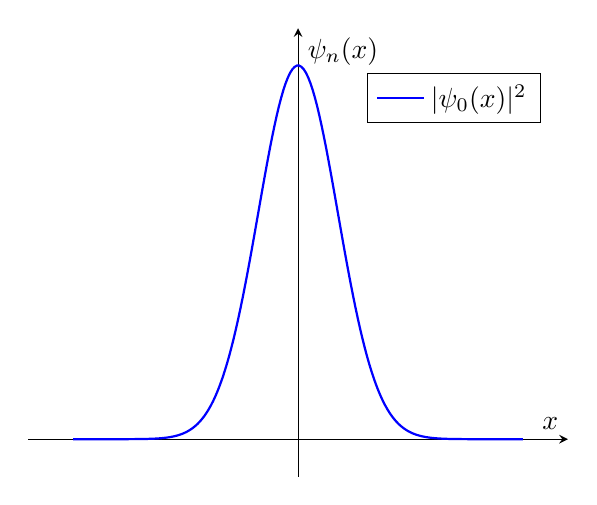
\begin{tikzpicture}
    \begin{axis}[
        axis lines = middle,
        xlabel = $x$,
        ylabel = $\psi_n(x)$,
        xtick=\empty,
        ytick=\empty,
        enlargelimits,
        legend style={at={(0.95,0.9)}, anchor=north east},
        domain = -4:4,
        samples = 200
    ]

    % Ground state |\psi_0|
    \addplot [blue, thick] {abs(pi^(-1/4)*exp(-x^2/2))^2};
    \addlegendentry{$|\psi_0(x)|^2$}
    \end{axis}
    
\end{tikzpicture}

\end{minipage}
%%%%%%%%
\vspace{1em}
%%%%%%%%
%%%  2  %%%	
%%%%%%%%
\vspace{1em}
%%%%%%%%
\begin{minipage}{0.5\textwidth}

\begin{tikzpicture}
    \begin{axis}[
        axis lines = middle,
        xlabel = $x$,
        ylabel = $\psi_n(x)$,
        enlargelimits,
        xtick=\empty,
        ytick=\empty,
        legend style={at={(0.95,0.9)}, anchor=north east},
        domain = -4:4,
        samples = 200
    ]

   % First excited state \psi_1
    \addplot [red, thick] {sqrt(2)*pi^(-1/4)*x*exp(-x^2/2)};
    \addlegendentry{$\psi_1(x)$}
    \end{axis}
    
\end{tikzpicture}

\end{minipage}
\hfill
\begin{minipage}{0.5\textwidth}

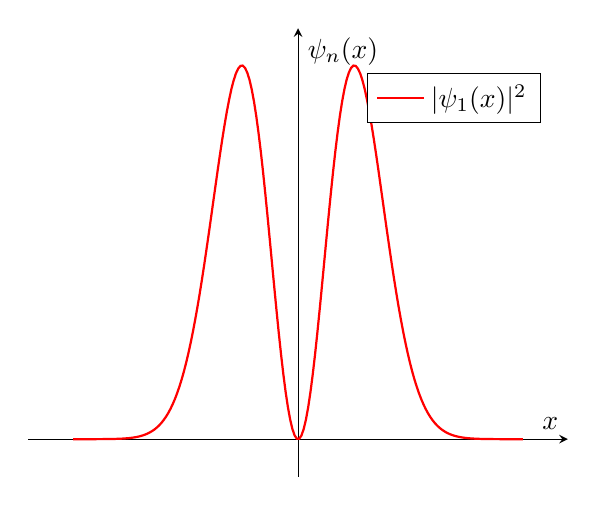
\begin{tikzpicture}
    \begin{axis}[
        axis lines = middle,
        xlabel = $x$,
        ylabel = $\psi_n(x)$,
        xtick=\empty,
        ytick=\empty,
        enlargelimits,
        legend style={at={(0.95,0.9)}, anchor=north east},
        domain = -4:4,
        samples = 200
    ]

     % First excited state |\psi_1|
    \addplot [red, thick] {abs(sqrt(2)*pi^(-1/4)*x*exp(-x^2/2))^2};
    \addlegendentry{$|\psi_1(x)|^2$}
    \end{axis}
    
\end{tikzpicture}

\end{minipage}
%%%%%%%%
\vspace{1em}
%%%%%%%%
%%%  3  %%%	
%%%%%%%%
\vspace{1em}
%%%%%%%%
\begin{minipage}{0.5\textwidth}

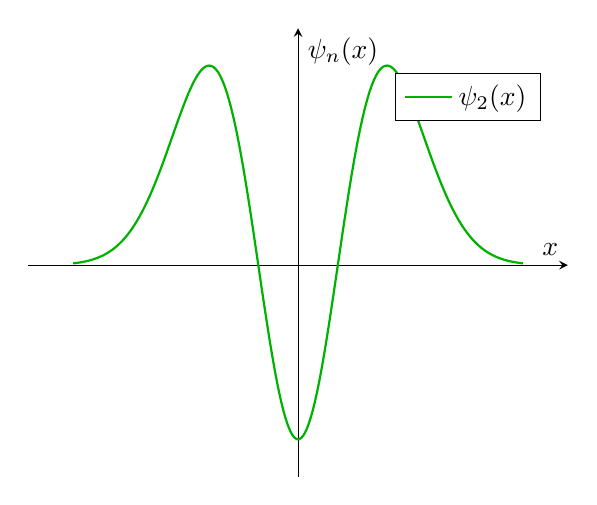
\begin{tikzpicture}
    \begin{axis}[
        axis lines = middle,
        xlabel = $x$,
        ylabel = $\psi_n(x)$,
        xtick=\empty,
        ytick=\empty,
        enlargelimits,
        legend style={at={(0.95,0.9)}, anchor=north east},
        domain = -4:4,
        samples = 200
    ]

   % Second excited state \psi_2
    \addplot [green!70!black, thick] {1/sqrt(2)*pi^(-1/4)*(2*x^2-1)*exp(-x^2/2)};
    \addlegendentry{$\psi_2(x)$}
    \end{axis}
    
\end{tikzpicture}

\end{minipage}
\hfill
\begin{minipage}{0.5\textwidth}

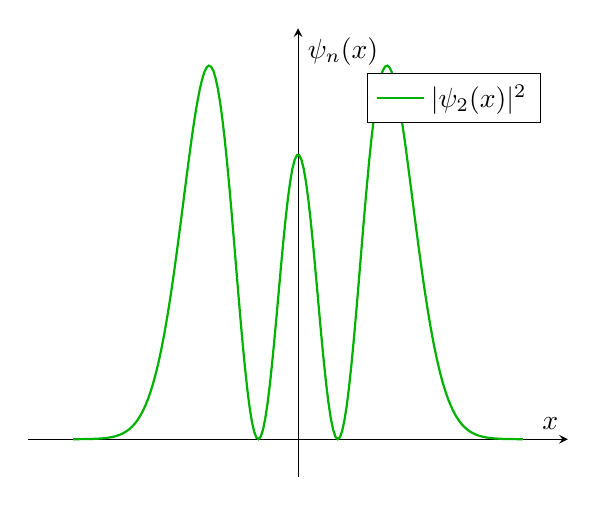
\begin{tikzpicture}
    \begin{axis}[
        axis lines = middle,
        xlabel = $x$,
        ylabel = $\psi_n(x)$,
        xtick=\empty,
        ytick=\empty,
        enlargelimits,
        legend style={at={(0.95,0.9)}, anchor=north east},
        domain = -4:4,
        samples = 200
    ]

     % Second excited state |\psi_2|
    \addplot [green!70!black, thick] {abs(1/sqrt(2)*pi^(-1/4)*(2*x^2-1)*exp(-x^2/2))^2};
    \addlegendentry{$|\psi_2(x)|^2$}
    \end{axis}
    
\end{tikzpicture}

\end{minipage}
%%%%%%%
\vspace{1em}
%%%%%%%

\subsection{Rappresentazione di Heisenberg}

\begin{nb}
	Si da il nome di rappresentazione di Heisenberg ad ogni rappresentazione in cui la matrice che rappresenta $\hat{H}$ è diagonale.
\end{nb}

	Nel caso dell'oscillatore armonico dunque, se la rappresentazione di $\hat{H}$ nella RH è \textit{ovvia}, ossia è diagonale, non sono così ovvie invece quelle di: $\hat{a}, \hat{a}^{\dagger}, \hat{x}, \hat{p}$. Ciò diventa chiaro dal momento in cui notiamo che siamo nella base dell'operatore numero e nessuno di questi quattro operatori commuta con esso. Possiamo allora proseguire a calcolare i termini delle matrici corrispondenti agli operatori di salita e discesa $\hat{a}^{\dagger}$ ed $\hat{a}$, dunque:
	
\begin{align*}
	&\qty(\hat{a}^{\dagger})_{nm} = \mel{n}{\hat{a}^{\dagger}}{m} = \mel{n}{\sqrt{m+1}}{m+1} = \sqrt{m+1} \braket{n}{m+1} = \delta_{n, \, m+1} \, \sqrt{m+1} \\
	& \qty(\hat{a})_{nm} = \mel{n}{\hat{a}}{m} = \mel{n}{\sqrt{m}}{m-1} = \sqrt{m} \braket{n}{m-1} = \delta_{n, \, m-1} \, \sqrt{m} = \delta_{n+1, \, m} \, \sqrt{n+1}
\end{align*}

	pertanto le due matrici sono:
	
\begin{align*}
	\hat{a}^{\dagger} = \mqty(0&0&0&0& \cdots \\ 1&0&0&0& \cdots \\ 0&\sqrt{2}&0&0& \cdots \\ 0&0&\sqrt{3}&0& \cdots \\ \vdots&\vdots&\vdots&\vdots& \ddots ) \qquad ; \qquad \hat{a} = {}^T \qty(\hat{a}^{\dagger})=  \mqty(0&1&0&0& \cdots \\0&0&\sqrt{2}&0& \cdots \\ 0&0&0&\sqrt{3}& \cdots \\ 0&0&0&0& \cdots \\\vdots&\vdots&\vdots&\vdots& \ddots )
\end{align*}

	esprimiamo allora gli operatori $\hat{x}$ ed $\hat{p}$ in termini di $\hat{a}$ ed $\hat{a}^{\dagger}$ ottenendo:

\begin{nb}
\begin{align*}
	&\hat{x} = - i \, \sqrt{\frac{\hbar}{2m\omega}} \, \qty(\hat{a}^{\dagger} - \hat{a}) \\
	&\hat{p} = \sqrt{\frac{m\hbar\omega}{2}} \,\qty(\hat{a}^{\dagger} + \hat{a})
\end{align*}
\end{nb}

	e dunque in forma di elemento matriciale:
	
\begin{align*}
	&\qty(\hat{x})_{nm} = - i \, \sqrt{\frac{\hbar}{2m\omega}} \mel{n}{\hat{a}^{\dagger} - \hat{a}}{m} = - i \, \sqrt{\frac{\hbar}{2m\omega}} \, \qty\Big(\delta_{n, \, m+1} \sqrt{m+1} - \delta_{n, \, m-1}\sqrt{m}) \\
	&\qty(\hat{p})_{nm} = \sqrt{\frac{m\hbar\omega}{2}} \mel{n}{\hat{a}^{\dagger} + \hat{a}}{m} = \sqrt{\frac{m\hbar\omega}{2}} \, \qty\Big( \delta_{n, \, m+1} \sqrt{m+1} + \delta_{n, \, m-1}\sqrt{m} )
\end{align*}

	ossia:
	
\begin{align*}
	\hat{x} = - i \, \sqrt{\frac{\hbar}{2m\omega}} \,\mqty(0&-1&0&0& \cdots \\ 1&0&-\sqrt{2}&0& \cdots \\ 0&\sqrt{2}&0&-\sqrt{3}& \cdots \\ 0&0&\sqrt{3}&0& \cdots \\ \vdots&\vdots&\vdots&\vdots& \ddots ) \qquad ; \qquad \hat{p} = \sqrt{\frac{m\hbar\omega}{2}} \,  \mqty(0&1&0&0& \cdots \\1&0&\sqrt{2}&0& \cdots \\ 0&\sqrt{2}&0&\sqrt{3}& \cdots \\ 0&0&\sqrt{3}&0& \cdots \\\vdots&\vdots&\vdots&\vdots& \ddots )
\end{align*}

	e dunque utilizzando le ultime due matrici nell'equazione per $\hat{H}$ dell'oscillatore armonico, trovo $\hat{H}$ in forma diagonale, con gli autovalori $E_n$ sulla diagonale, ovvero:
	
\begin{align*}
	\hat{H} = \frac{1}{2} \, \hbar \omega \,  \mqty(1&0&0&0&0&  \cdots \\0&3&0&0&0&  \cdots \\ 0&0&5&0&0&  \cdots \\ 0&0&0&7&0&  \cdots \\ 0&0&0&0&9&  \cdots \\\vdots&\vdots&\vdots&\vdots&\vdots&  \ddots )
\end{align*}	

\subsection{Stati Coerenti}

	In questa sezione trattiamo gli \textit{stati coerenti} in relazione all'oscillatore armonico quantistico. Vediamone subito la definizione:
	
\begin{mydef}
	Uno \textbf{stato coerente} $\ket{\alpha}$ è definito come un autostato dell'operatore di distruzione $\hat{a}$:
\begin{align*}
	\hat{a}\ket{\alpha} = \alpha \ket{\alpha}
\end{align*}
\end{mydef}

	poiché $\hat{a}$ non è hermitiano, in generale $\alpha \in \mathbb{C}$. 
	\\
	\\
	Cosa significa concettualmente che gli stati coerenti sono autostati dell'operatore di distruzione?
	\\
	\\
	Come sappiamo un autostato è uno stato "speciale" che non cambia, nel senso proprio del termine, ovvero che quando gli si applica l'operatore corrispondente, viene solo riscalato di un fattore, l'autovalore. Siccome $\hat{a}$ rimuove quanti di energia, ci chiediamo come gli autostati e la funzione di operatore di discesa siano collegati. Costruisco un'espressione esplicita per gli stati coerenti che possa dare un senso a quanto appena detto. Per fare ciò scriveremo gli stati coerenti nella base degli autostati dell'Hamiltoniana. In termini degli autostati dell'oscillatore armonico quantistico nella base dell'energia si ha:
	
\begin{align*}
	\hat{H} \ket{n} = E_n \ket{n} 
\end{align*}
	
	quindi possiamo scrivere $\ket{n}$ nella base $\ket{\alpha}$ come:
	
\begin{align*}
	\ket{\alpha} = \sum_{n = 0}^{\infty} \ket{n} \braket{n}{\alpha} = \sum_{n=0}^{\infty} c_n \ket{n}
\end{align*}
	
	con: $c_n = \braket{n}{\alpha}$. Quindi applicando $\hat{a}$ si ottiene che:
	
\begin{align*}
	\hat{a} \ket{\alpha} = \hat{a} \, \sum_{n = 0}^{\infty} c_n \ket{n} = \sum_{n=0}^{\infty} c_n \, \hat{a} \ket{n}
\end{align*}
	
	ricordiamo inoltre che è inutile partire da $ n = 0$ poiché l'azione di $\hat{a}$ su $\ket{0}$ è $0$, allora si parte da $n = 1$, ricordiamo inoltre che vale:
	
\begin{align*}
	\hat{a} \ket{n} = \sqrt{n} \ket{n-1} 
\end{align*}

	dunque:
	
\begin{align*}
	\hat{a} \ket{\alpha} = \sum_{n = 1}^{\infty} c_n \, \sqrt{n} \ket{n-1} 
\end{align*}
	
	per comodità: \textit{rinomino l'indice} $n \to n +1$, allora: 
	
\begin{align*}
	\hat{a} \ket{\alpha} = \sum_{n +1 = 1}^{\infty} c_{n +1} \, \sqrt{n +1} \ket{n +1-1} = \sum_{n = 0}^{\infty} c_{n +1} \, \sqrt{n +1} \ket{n} 
\end{align*}
	
	ricordando ora la definizione di \textit{stato coerente:}
	
\begin{align*}
	\hat{\alpha} = \alpha \ket{\alpha} 
\end{align*}
	
	allora:

\begin{align*}
	\textcolor{blue}{\hat{\alpha}} = \alpha \textcolor{orange}{\ket{\alpha} } \Leftrightarrow \, \textcolor{blue}{\sum_{n = 0}^{\infty} c_{n +1} \, \sqrt{n +1} \ket{n}}  = \alpha \textcolor{orange}{\sum_{n = 0}^{\infty} c_n \ket{n} }
\end{align*}
	
	allora porto tutto a sinistra:
	
\begin{align*}
	\sum_{n = 0}^{\infty} \qty\Big(c_{n +1} \, \sqrt{n +1} \ket{n} - \alpha \, c_n \ket{n}) = 0 \, \Rightarrow \, \sum_{n = 0}^{\infty} \qty\Big(c_{n +1} \, \sqrt{n +1} - \alpha \, c_n ) \ket{n} = 0 
\end{align*}

	l'espressione che abbiamo ottenuto è dunque vera se il termine dentro la somma è nullo. Otteniamo in questo modo una relazione di ricorrenza per $c_{n+1}$ in termini di $c_n$:
	
\begin{align*}
	c_{n +1} \, \sqrt{n +1} - \alpha \, c_n = 0\, \Rightarrow \, c_{n+1} = \frac{\alpha}{\sqrt{n+1}} \, c_n
\end{align*}
	
	si tratta dunque di una relazione che lega ogni $c_{n+1}$ con il precedente $c$, essendo che tale relazione è vera $\forall n$ posso scrivere $c_n$ in termini di $c_{n-1}$ e così via. Usando dunque $c_n$ come termine di partenza e iterando fino a $c_0$ si ha:
	
\begin{align*}
	c_n = \frac{\alpha}{\sqrt{n}} \,\textcolor{blue}{c_{n-1}}
\end{align*}
	
	possiamo riapplicare la stessa cosa a $c_{n-1}$, ovvero:
	
\begin{align*}
	\textcolor{blue}{c_{n-1}} =  \frac{\alpha}{\sqrt{n-1}} \, c_{n-2}
\end{align*}

	e allora, appunto, iterando questa sostituzione fino a $c_0$:

\begin{align*}
	c_n = \frac{\alpha}{\sqrt{n}} \, \frac{\alpha}{\sqrt{n-1}} \, \cdots \, \frac{\alpha}{\sqrt{2}} \, \frac{\alpha}{\sqrt{1}} \, c_0 = \frac{\alpha^n}{\sqrt{n!}} \, c_0
\end{align*}
	
	pertanto possiamo sostituire nello stato coerente:
	
\begin{align*}
	\ket{\alpha} = \sum_{n = 0}^{\infty} \textcolor{ForestGreen}{c_n} \ket{n} = \sum_{n= 0}^{\infty} \textcolor{ForestGreen}{\frac{\alpha^n}{\sqrt{n!}} \, c_0} \ket{n} 
\end{align*}
	
	mi basta dunque ora determinare chi sia $c_0$. Ciò si può fare normalizzando gli stati. Impongo allora:
	
\begin{align*}
	1 = \sum_{n = 0}^{\infty} |c_n|^2 =  \sum_{n = 0}^{\infty} \abs{\frac{\alpha^n}{\sqrt{n!}}}^2 \, |c_0|^2 = |c_0|^2 \textcolor{red}{\sum_{n = 0}^{\infty} \frac{|\alpha|^{2n}}{n!}}
\end{align*}

	Riconosco subito che la sommatoria è proprio l'espansione in serie di potenze dell'esponenziale di $|\alpha|^2$, ovvero:
	
\begin{align*}
	\textcolor{red}{e^{ |\alpha|^2} } = \sum_{n = 0}^{\infty} \frac{|\alpha|^{2n}}{n!}
\end{align*}

	allora:
	
\begin{align*}
	1 = |c_0|^2 \, e^{ |\alpha|^2} \, \Rightarrow \, |c_0|^2  = e^{\, - |\alpha|^2} \, \Rightarrow \, c_0  = e^{\, - |\alpha|^2/2} 
\end{align*}

	perciò da:

\begin{align*}
	\ket{\alpha} = \sum_{n= 0}^{\infty} \frac{\alpha^n}{\sqrt{n!}} \, c_0 \ket{n} = \textcolor{blue}{c_0} \sum_{n= 0}^{\infty} \frac{\alpha^n}{\sqrt{n!}} \ket{n} = \textcolor{blue}{e^{\, - |\alpha|^2/2} } \sum_{n= 0}^{\infty} \frac{\alpha^n}{\sqrt{n!}} \ket{n} 
\end{align*}

	Il risultato finale può essere espresso anche in termini dello stato iniziale $\ket{0}$, infatti ricordando il risultato ottenuto con la rappresentazione olomorfa per i livelli energetici, si ha che, preso il "ground state" allora possiamo ricavare tutti gli altri livelli con:
	
\begin{align*}
	\ket{n} = \frac{\qty(\hat{a}^{\dagger})^n}{\sqrt{n!}} \ket{0}
\end{align*}

	allora possiamo riscrivere $\ket{\alpha}$ come:

\begin{align*}
	\ket{\alpha} = e^{\, - |\alpha|^2/2}  \sum_{n= 0}^{\infty} \frac{\alpha^n}{\sqrt{n!}} \textcolor{orange}{\ket{n}} = e^{\, - |\alpha|^2/2}  \sum_{n= 0}^{\infty} \frac{\alpha^n}{\sqrt{n!}} \textcolor{orange}{  \frac{\qty(\hat{a}^{\dagger})^n}{\sqrt{n!}} \ket{0} } = e^{\, - |\alpha|^2/2}  \sum_{n= 0}^{\infty}\frac{\qty(\alpha \, \hat{a}^{\dagger})^n}{n!} \ket{0} 
\end{align*}

	dove notiamo che, come prima:
	
\begin{align*}
	\sum_{n= 0}^{\infty}\frac{\qty(\alpha \, \hat{a}^{\dagger})^n}{n!} \quad \Rightarrow \quad \text{è l'espansione in serie di potenze di $e^{\alpha \, \hat{a}^{\dagger}}$}
\end{align*}

	allora:

\begin{align*}
	\ket{\alpha} = e^{\, - |\alpha|^2/2}  \sum_{n= 0}^{\infty}\frac{\qty(\alpha \, \hat{a}^{\dagger})^n}{n!} \ket{0}  = e^{\, - |\alpha|^2/2} \, e^{\alpha \, \hat{a}^{\dagger}} \ket{0} 
\end{align*}
	
	ovvero:

\begin{nb}
\begin{align*}
	\ket{\alpha} = e^{\, - |\alpha|^2/2} \, e^{\alpha \, \hat{a}^{\dagger}} \ket{0} = e^{\, - |\alpha|^2/2} \sum_{n = 0}^{\infty} \frac{\alpha^n}{\sqrt{n!}} \ket{n}
\end{align*}
\end{nb}
	
	Allora possiamo fare delle osservazioni su questo risultato. Per rispondere alla domanda iniziale, lo stato coerente ricavato è una sovrapposizione di tutti i possibili autostati dell'energia $\ket{n}$, quindi essenzialmente una sovrapposizione di un numero infinito di autostati dell'energia. Quando facciamo agire $\hat{a}$ sullo stato $\ket{\alpha}$, ad ogni  termine della somma rimuoviamo un quanto di energia, ma la forma del coefficiente di espansione è tale che ogni termine diventa esattamente uguale al termine originale con un quanto di energia in meno, cosicché complessivamente lo stato non cambia. Ciò è dato dal fatto che la somma è infinita, quindi non esiste qualcosa come "uno stato di energia massima" che non potremmo raggiungere dopo aver fatto agire $\hat{a}$. In altre parole, il risultato finale dell’operazione è che lo stato coerente rimane lo stesso stato coerente, moltiplicato semplicemente per il numero $\alpha$:
	
\begin{align*}
	\hat{a} \ket{\alpha} = \alpha \ket{\alpha}
\end{align*}

	Questo risultato è molto importante, perché ci dice che lo stato coerente è un autostato dell’operatore di annichilazione con autovalore $\alpha$. 
	\\
	\\
	La chiave è, appunto, nell’infinità della somma: poiché la somma non ha un limite superiore (cioè non c’è uno stato massimo oltre il quale non si può andare), applicare $\hat{a}$ non "termina" mai la sequenza. Se avessimo un numero finito di termini (come in un caso limite), a un certo punto arriverebbe a zero, e lo stato cambierebbe drasticamente. Ma nello stato coerente abbiamo infiniti termini, quindi l'operatore $\hat{a}$:
	
\begin{itemize}
	\item "sposta" semplicemente i coefficienti della serie, ridistribuendoli in modo che la struttura infinita rimanga identica.
	\item pertanto, non si raggiunge mai uno stato "finale": ogni volta che si toglie un quanto di energia a uno stato, ce n’è sempre un altro pronto a prendere il suo posto nella somma infinita.
\end{itemize}
	
	Quindi lo stato rimane formalmente invariato nella sua struttura infinita.
	
\subsubsection{Livelli energetici degli stati coerenti:}
	
	Consideriamo dunque un oscillatore armonico nello stato $\ket{\alpha}$. Per quanto detto prima, la probabilità che questo abbia energia pari a:
	
\begin{align*}
	E_n = \hbar \omega \, \qty(n + \frac{1}{2})
\end{align*}

	deve essere:
	
\begin{align*}
	P_n(\alpha) = |c_n(\alpha)|^2
\end{align*}

\begin{myapprf}
	Per la formula della probabilità ricordiamo che: la probabilità di misurare un particolare autostato del sistema (in questo caso, uno specifico livello energetico $E_n$) è uguale al modulo quadro del coefficiente che moltiplica quell'autostato nell'espansione dello stato iniziale sulla base degli autostati misurati. Ovvero, detto esplicitamente, dato lo stato:

\begin{align*}
	\ket{\psi} = \sum_n c_n \ket{n}
\end{align*}

	allora la probabilità di misurare il sistema nello stato $\ket{n}$ è:
	
\begin{align*}
	P_n = |c_n|^2
\end{align*}
\end{myapprf}

	essendo che sappiamo che:
	
\begin{align*}
	c_n(\alpha) = \frac{\alpha^n}{\sqrt{n!}} c_0 = \frac{\alpha^n}{\sqrt{n!}} \, e^{\, - |\alpha|^2/2}  
\end{align*}

	allora:
	
\begin{align*}
	P_n(\alpha) = |c_n(\alpha)|^2 = \frac{|\alpha|^{2n}}{n!} \, e^{\, -|\alpha|^2}
\end{align*}

	la distribuzione di probabilità ottenuta è dunque una distribuzione Poissoniana. Calcoliamo ora il valore di aspettazione dell'Hamiltoniana sullo stato coerente $\ket{\alpha}$ che è definito come:
	
\begin{align*}
	\mel{\alpha}{\hat{H}}{\alpha} \, \equiv \, \mean{\hat{H}}_{\alpha} 
\end{align*}

	ricordiamo che:

\begin{align*}
	E_n = \hbar \omega \, \qty(n + \frac{1}{2})
\end{align*}

	che è  l’energia del livello $n$-esimo dell’oscillatore armonico.
	\\
	\\
	Si calcola allora il valore di aspettazione esplicitamente:
	
\begin{align*}
	\mean{\hat{H}}_{\alpha} = \mel{\alpha}{\hat{H}}{\alpha} = \sum_n \braket{\alpha}{n} \mel{n}{\hat{H}}{\alpha}
\end{align*}
	
	e sapendo che:
	
\begin{align*}
	\hat{H} \ket{n} = E_n \ket{n}
\end{align*}

	allora:
	
\begin{align*}
	\mel{n}{\hat{H}}{\alpha} = E_n \braket{n}{\alpha}
\end{align*}

	sostituendo:
	
\begin{align*}
	\mean{\hat{H}}_{\alpha} = \sum_n \braket{\alpha}{n} \mel{n}{\hat{H}}{\alpha} = \sum_n \braket{\alpha}{n} E_n \braket{n}{\alpha} = \sum_n E_n \, |\braket{\alpha}{n}|^2
\end{align*}
	
	e sapendo:
	
\begin{align*}
	P_n(\alpha) = |\braket{\alpha}{n}|^2
\end{align*}
	
	allora:

\begin{align*}
	\mean{\hat{H}}_{\alpha} = \mel{\alpha}{\hat{H}}{\alpha} = \sum_n P_n(\alpha) \, \hbar \omega \, \qty( n + \frac{1}{2})
\end{align*}

	notiamo ora che:
	
\begin{align*}
	\sum_n P_n \, n = \sum_n |\braket{n}{\alpha}|^2 \, n
\end{align*}

	ricordando che $n$ è l’autovalore dell’operatore $\hat{n} = \hat{a}^{\dagger}\hat{a} $ associato allo stato $\ket{n}$, quindi stiamo facendo la media pesata degli autovalori dell’operatore numero $\hat{n}$ secondo le probabilità $P_n(\alpha)$, e sappiamo che vale in generale
	
\begin{align*}
	\mean{\hat{O}} = \sum_n |\braket{n}{\psi}|^2 \, o_n
\end{align*}

	dove $o_n$ sono gli autovalori di $\hat{O}$ e $\ket{n}$ i suoi autostati. Allora nel nostro caso:

\begin{align*}
	\mean{\hat{n}} = \sum_n |\braket{n}{\alpha}|^2 \, n = \sum_n P_n(\alpha) \, n 
\end{align*}

	infatti vale che:
	
\begin{align*}
	\mean{\hat{n}} = \mean{\hat{a}^{\dagger}\hat{a}} = \mel{\alpha}{\hat{a}^{\dagger}\hat{a}}{\alpha}
\end{align*}

	e quindi mettendo insieme le cose:
	
\begin{align*}
	\sum_n P_n(\alpha) \, n = \mel{\alpha}{\hat{a}^{\dagger}\hat{a}}{\alpha}
\end{align*}

	allora possiamo tornare indietro e dire:
	
\begin{align*}
	\mean{\hat{H}}_{\alpha} = \sum_n P_n(\alpha) \hbar \omega \, \qty(n+\frac{1}{2}) =  \hbar \omega \, \qty( \textcolor{blue}{\sum_n P_n(\alpha) \, n} +\frac{1}{2}) = \hbar \omega \, \qty( \textcolor{blue}{\mel{\alpha}{\hat{a}^{\dagger}\hat{a}}{\alpha}} +\frac{1}{2}) 
\end{align*}

	ricaviamoci dunque ora esplicitamente il valore di aspettazione di $\hat{a}{\dagger}\hat{a}$, infatti possiamo notare:
	
\begin{align*}
	& \bra{\alpha} \hat{a}^{\dagger} = \alpha^* \bra{\alpha} \\
	& \hat{a} \ket{\alpha} = \alpha \ket{\alpha}
\end{align*}

	e dunque si ha:
	
\begin{align*}
	\mel{\alpha}{\hat{a}^{\dagger}\hat{a}}{\alpha} = \alpha^* \alpha \braket{\alpha}
\end{align*}

	ed essendo $\ket{\alpha}$ normalizzato allora:
	
\begin{align*}
	\mel{\alpha}{\hat{a}^{\dagger}\hat{a}}{\alpha} = \alpha^* \alpha 
\end{align*}

	e dunque infine:

\begin{nb}
\begin{align*}
	\mean{\hat{H}}_{\alpha} = \hbar \omega \, \qty( \textcolor{blue}{\mel{\alpha}{\hat{a}^{\dagger}\hat{a}}{\alpha}} +\frac{1}{2}) = \hbar \omega \, \qty( \textcolor{blue}{\alpha^* \alpha} +\frac{1}{2}) = \hbar \omega \, \qty( |\alpha|^2 +\frac{1}{2}) 
\end{align*}
\end{nb}
	
\subsubsection{Valori medi ed incertezze di posizione ed impulso su stati coerenti:}
	
	Possiamo ottenere i valori di $\mean{\hat{x}}$, $\mean{\hat{p}}$ sullo stato coerente, scrivendoli in termini degli operatori di creazione e distruzione. Si ottengono seguendo un calcolo analogo al precedente, ovvero, ricordando prima di tutto che:
	
\begin{nb}
	L'operatore di posizione e momento si possono scrivere in funzione degli altri operatori come:
\begin{align*}
	& \hat{x} = \sqrt{\frac{\hbar}{2m\omega}} \, \qty(\hat{a}^{\dagger} + \hat{a})\\
	& \hat{p} = i \, \sqrt{\frac{m\hbar\omega}{2}} \, \qty(\hat{a}^{\dagger} - \hat{a})
\end{align*}
\end{nb}
	
	ricordando inoltre che lo stato coerente è autostato dell'operatore $\hat{a}$, ovvero tale che:
	
\begin{align*}
	\hat{a} \ket{\alpha} = \alpha \ket{\alpha} \qquad ; \qquad \bra{\alpha} \hat{a}^{\dagger} = \alpha^* \bra{\alpha}
\end{align*}
	
	e quindi:
	
\begin{align*}
	& \mean{\hat{x}}_{\alpha} = \mel{\alpha}{\hat{x}}{\alpha} = \sqrt{\frac{\hbar}{2m\omega}} \, \qty\Big(\mel{\alpha}{\hat{a}^{\dagger}}{\alpha} + \mel{\alpha}{\hat{a}}{\alpha})  \\
	& \mean{\hat{p}}_{\alpha} = \mel{\alpha}{\hat{p}}{\alpha} = i \, \sqrt{\frac{m\hbar\omega}{2}} \, \qty\Big(\mel{\alpha}{\hat{a}^{\dagger}}{\alpha} - \mel{\alpha}{\hat{a}}{\alpha})
\end{align*}

	dove sappiamo valere:
	
\begin{align*}
	\mel{\alpha}{\hat{a}}{\alpha}) = \alpha \qquad ; \qquad \mel{\alpha}{\hat{a}^{\dagger}}{\alpha} = \alpha^*
\end{align*}

	allora:
	
\begin{align*}
	& \mean{\hat{x}}_{\alpha} = \sqrt{\frac{\hbar}{2m\omega}} \, \qty\Big( \alpha^*+  \alpha)  \\
	& \mean{\hat{p}}_{\alpha} = i \, \sqrt{\frac{m\hbar\omega}{2}} \, \qty\Big( \alpha^* -  \alpha)
\end{align*}

	notiamo che:
	
\begin{align*}
	& \textcolor{orange}{\alpha} +\textcolor{Magenta}{ \alpha^*} = \textcolor{orange}{a + ib} + \textcolor{Magenta}{a - ib} = 2a \, \equiv \, 2 \Re(\alpha) \\
	& \alpha^* - \alpha = a - ib - \qty(a + ib) = a - ib - a - ib = -2ib = - i \, 2 b \, \equiv \,  - i \,  2 \Im(\alpha)
\end{align*}

	allora:

\begin{align*}
	& \mean{\hat{x}}_{\alpha} = \sqrt{\frac{\hbar}{2m\omega}} \, 2 \Re(\alpha) =  \sqrt{\frac{2\hbar}{m\omega}} \Re(\alpha) \\
	& \mean{\hat{p}}_{\alpha} = i \, \sqrt{\frac{m\hbar\omega}{2}} \, \qty\Big(- i \, 2 \Im(\alpha)) =  \sqrt{2m\hbar\omega} \, \Im(\alpha)
\end{align*}

	abbiamo dunque ottenuto:

\begin{mydef}
	Il \textbf{valore di aspettazione} degli operatori $\hat{x}, \hat{p}$ sullo stato coerente è pari a:
\begin{align*}
	& \mean{\hat{x}}_{\alpha} =\sqrt{\frac{2\hbar}{m\omega}} \, \Re (\alpha) \\
	&  \mean{\hat{p}}_{\alpha} = \sqrt{2m\hbar \omega} \, \Im (\alpha)
\end{align*}
\end{mydef}

	e calcoli analoghi portano a:

\begin{mydef}
	Si possono ricavare i \textbf{valori di aspettazione dei quadrati degli operatori} allo stesso modo:
\begin{align*}
	& \mean{\hat{x}^2}_{\alpha} = \frac{\hbar}{2m\omega} \, \qty\Big[\qty(\alpha + \alpha^*)^2 + 1 ] \\
	& \mean{\hat{p}^2}_{\alpha} = \frac{m\hbar\omega}{2} \, \qty\Big[ 1 - \qty(\alpha - \alpha^*)^2 ] \\
	& \mean{\hat{H}^2}_{\alpha}  = \hbar^2 \omega^2 \, \qty\Big( |\alpha|^4 + 2 \, |\alpha|^2 + \frac{1}{4} )
\end{align*}
\end{mydef}

	Inoltre, ricordando che in generale vale:
	
\begin{align*}
	\Delta \hat{O} = \sqrt{\mean{O^2} - \mean{O}^2}
\end{align*}

	allora si trovano le  rispettive incertezze che sono:

\begin{mydef}
	Utilizzando le formule cui sopra, si trovano le \textbf{incertezze} che valgono allora:
\begin{align*}
	& \Delta \hat{x}_{\alpha} = \sqrt{\frac{\hbar}{2m\omega}}  \\
	& \Delta\hat{p}_{\alpha} = \sqrt{\frac{m\hbar\omega}{2}} \\
	& \Delta \hat{H}_{\alpha} = \hbar \omega \, |\alpha|
\end{align*}
\end{mydef}

	da queste espressioni possiamo notare come né $\Delta \hat{x}_{\alpha}$ né $\Delta \hat{p}_{\alpha}$ dipendono dallo stato coerente $\alpha$. Si nota inoltre che abbiamo ottenuto che gli stati coerenti sono stati di \textbf{minima indeterminazione}, infatti:
	
\begin{align*}
	\Delta \hat{x} \Delta \hat{p} = \frac{\hbar}{2}
\end{align*}
	
\subsubsection{Valore medio del momento angolare orbitale su uno stato coerente:}

	Ricordiamo che, in meccanica quantistica, gli stati coerenti sono stati speciali del sistema oscillatore armonico quantistico che si comportano "quasi classicamente". In 1D sono della forma:
	
\begin{align*}
	\ket{\alpha} = e^{\, \alpha a^{\dagger}} \ket{0}
\end{align*}

	Considero lo stato coerente non normalizzato in tre dimensioni:

\begin{align*}
	\ket{\psi} = e^{\, \sum_{i=1}^3 \alpha a_i^{\dagger}} \ket{0} = e^{\, \vb*{\alpha} \vdot \vb*{a}^{\dagger}} \ket{0} \, \equiv \, \hat{U}(\alpha) \ket{0}
\end{align*}

	e cerchiamo il valore medio della componente $i$-esima del momento angolare orbitale $L_i$, su questo stato. Diciamo dunque che abbiamo questo operatore lineare traslante (l'operatore unitario) definito come: 

\begin{align*}
	\hat{U}(\alpha) \, \equiv \, e^{\, \vb*{\alpha} \vdot \vb*{a}^{\dagger}}
\end{align*}

	e vogliamo allora calcolare come agisce su un operatore $L_i$ per "coniugazione", ovvero:
	
\begin{align*}
	U^{-1}(\alpha) \, L_i \, U(\alpha) 
\end{align*}

	In meccanica quantistica, capita spesso di voler sapere come un operatore cambia quando applico una trasformazione unitaria. Il trucco, come abbiamo precedentemente visto, è espandere la trasformazione in serie di commutatori, ed è qui che entra in gioco questa identità che in generale è:
	
\begin{align*}
	e^{\, - A} \, B \, e^{A} = B - \qty[A, B] + \frac{1}{2!} \, \qty\Big[A, \qty[A, B] ]- \frac{1}{3!} \, \ldots
\end{align*}
	
	allora fissando:

\begin{itemize}
	\item $A = \vb*{\alpha} \vdot \vb{a}^{\dagger}$, 
	\item $B = L_i$
\end{itemize}
	
	si ottiene:
	
\begin{align*}
	 U^{-1}(\alpha) \, L_i \, U(\alpha)  = L_i - \qty\Big[\vb*{\alpha} \vdot \vb*{a}^{\dagger}, L_i ] + \frac{1}{2} \, \qty\Big[\vb*{\alpha} \vdot \vb{a}^{\dagger}, \qty\big[\vb*{\alpha} \vdot \vb*{a}^{\dagger}, L_i]] + \ldots
\end{align*}
	
	e poiché:
	
\begin{align*}
	&\qty\Big[L_i, \vb*{\alpha} \vdot \vb*{a}^{\dagger}] = \qty\Big[L_i, \alpha_j \, a_j^{\dagger}]  = \alpha_j \, \qty\Big[L_i, \, a_j^{\dagger}]  \, \equiv \, i\hbar \, \varepsilon_{ijk} \, \alpha_j \, a_k^{\dagger} = i \hbar \, \qty(\vb*{\alpha} \cp \vb{a}^{\dagger})_i \\
	& \qty\Big[\vb*{\alpha} \vdot \vb{a}^{\dagger}, \qty\big[\vb*{\alpha} \vdot \vb*{a}^{\dagger}, L_i]] = \qty\Big[\vb*{\alpha} \vdot \vb*{a}^{\dagger}, - i\hbar \, \qty(\vb*{\alpha} \cp \vb{a}^{\dagger})_i ] = 0
\end{align*}

	si ha allora che:
	
\begin{align*}
	 U^{-1}(\alpha) \, L_i \, U(\alpha)  = L_i + i \hbar \qty(\vb*{\alpha} \cp \vb{a}^{\dagger})_i
\end{align*}

	da cui:

\begin{align*}
	L_i U(\alpha) = U(\alpha) \, \qty\Big[L_i  + i \hbar \qty(\vb*{\alpha} \cp \vb{a}^{\dagger})_i]
\end{align*}

	ed essendo:
	
\begin{align*}
	U(\alpha)\ket{0} \, \equiv \, \ket{\psi}
\end{align*}

	allora:
	
\begin{align*}
	L_i \, U(\alpha) \ket{0} = U(\alpha) \, \qty\Big[L_i  + i \hbar \qty(\vb*{\alpha} \cp \vb{a}^{\dagger})_i] \ket{0} \, \Rightarrow \, L_i \ket{\psi} = U(\alpha) \, \qty\Big[L_i  + i \hbar \qty(\vb*{\alpha} \cp \vb{a}^{\dagger})_i] \ket{0} 
\end{align*}

	allora possiamo continuare a semplificare e dire:
	
\begin{align*}
	 L_i \ket{\psi} = U(\alpha) \, \qty\Big[L_i  + i \hbar \qty(\vb*{\alpha} \cp \vb{a}^{\dagger})_i] \ket{0} = U(\alpha) \, L_i \ket{0} + U(\alpha) \, \qty\Big[  i\hbar \, \qty(\vb*{\alpha} \cp \vb{a}^{\dagger})_i ] \ket{0} =  0 + i \hbar \, \qty(\vb*{\alpha} \cp \vb*{a}^{\dagger})_i \ket{\psi} = i \hbar \, \qty(\vb*{\alpha} \cp \vb*{a}^{\dagger})_i \ket{\psi}
\end{align*}

	e quindi abbiamo ottenuto che:
	
\begin{mydef}
	L'\textbf{applicazione del momento angolare sullo stato coerente} abbiamo dimostrato essere: 
\begin{align*}
	 L_i \ket{\psi} = i \hbar \, \qty(\vb*{\alpha} \cp \vb*{a}^{\dagger})_i \ket{\psi}
\end{align*}
\end{mydef}

	perché $U(\alpha) L_i \ket{0}$ è nullo? perché ricordiamo che:

\begin{nb}
\begin{align*}
	L_i = i \hbar \, \varepsilon_{ijk} a_j^{\dagger} a_k
\end{align*}
\end{nb}
	
	e

\begin{align*}
	\hat{a} \ket{0} = 0 \, \Rightarrow \, a_k \ket{0} = 0
\end{align*}

	ne segue che:

\begin{nb}
\begin{align*}
	L_i \ket{0} = 0
\end{align*}
\end{nb}
	
	questo risultato è importante non solo perché permette di semplificare il risultato, ma anche perché ci sta dicendo che vuoto è uno stato totalmente simmetrico (invariante sotto rotazioni) e non possiede eccitazioni che possano conferirgli un momento angolare non nullo.
	\\
	\\
	Osserviamo quindi adesso che, per definizione uno stato coerente è autostato dell'operatore di distruzione:
	
\begin{align*}
	\vb{a} \ket{\psi} = \vb*{\alpha} \ket{\psi}
\end{align*}

	pertanto possiamo calcolare il valore di aspettazione dell'operatore di distruzione, infatti:
	
\begin{align*}
	\bra{\psi} \vb{a}^{\dagger} = \bra{\psi} \vb*{\alpha}^*
\end{align*}

	allora:
	
\begin{align*}
	\mel{\psi}{\vb*{a}^{\dagger}}{\psi} = \bra{\psi} \vb*{\alpha}^* \ket{\psi} = \vb*{\alpha}^* \braket{\psi}
\end{align*}

	considerato che per ipotesi $\ket{\psi}$ non è normalizzato. Allora possiamo calcolare anche il valore di aspettazione (il valore medio) del momento angolare, ovvero:
	
\begin{align*}
	\mel{\psi}{L_i}{\psi} = \bra{\psi} i \hbar \, \qty(\vb*{\alpha} \cp \vb*{a}^{\dagger})_i \ket{\psi} = i\hbar \qty(\vb*{\alpha} \cp \vb*{\alpha}^* )_i \braket{\psi}
\end{align*}

	allora ricaviamo il valore medio di $L_i$:

\begin{mydef}
	Il \textbf{valore di aspettazione del momento angolare sullo stato coerente} equivale a: 
\begin{align*}
	\mean{L_i} = \frac{\mel{\psi}{L_i}{\psi}}{\braket{\psi}} = i \hbar \qty(\vb*{\alpha} \cp \vb*{\alpha}^*)_i = i \hbar \, \varepsilon_{ijk} \alpha_j \alpha_k^*
\end{align*}
\end{mydef}

\subsubsection{L'Operatore $\hat{D}(\alpha)$: la funzione d'onda $\psi_{\alpha}(x)$ }

\begin{mydef}
	Si consideri l'operatore $\hat{D}(\alpha)$ che è definito come:
\begin{align*}
	\hat{D}(\alpha) = e^{\, \alpha \hat{a}^{\dagger} - \alpha^* \hat{a}}
\end{align*}
\end{mydef}

	questo operatore è unitario, infatti se ne calcoliamo l'aggiunta troviamo:

\begin{align*}
	\hat{D}^{\dagger}(\alpha) = e^{\, \alpha^* \hat{a} - \alpha \hat{a}^{\dagger}} 
\end{align*}	

	da cui:
	
\begin{align*}
	\hat{D}(\alpha) \, \hat{D}^{\dagger}(\alpha) = \hat{D}^{\dagger}(\alpha) \, \hat{D}(\alpha) = \mathbb{I}
\end{align*}

	dal momento che:
	
\begin{align*}
	\qty[\alpha \hat{a}^{\dagger}, - \alpha^* \hat{a}]  = \alpha^* \alpha
\end{align*}

	che è un numero e quindi possiamo usare la notazione introdotta precedentemente per il prodotto di due operatori esponenziali e scrivere:
	
\begin{align*}
	\hat{D}\qty(\alpha) = e^{\frac{- |\alpha|^2}{2}} e^{\alpha \hat{a}^{\dagger}} e ^{-\alpha^* \hat{a}}
\end{align*}

	Adesso calcoliamo allora il ket $\hat{D}\qty(\alpha) \ket{\varphi_0}$. Poiché:
	
\begin{align*}
	e^{- \alpha^* \hat{a}} \ket{\varphi_0} = \qty(1 - \alpha^* \hat{a} +\frac{\qty(\alpha^*)^2}{2!} \hat{a}^2 + \dots) \ket{\varphi_0} 
\end{align*}
	
	allora:
	
\begin{align*}
	\hat{D}\qty(\alpha) \ket{\varphi_0} &= e^{\frac{- |\alpha|^2}{2}} e^{\alpha \hat{a}^{\dagger}} \ket{\varphi_0} \\
	& =  e^{\frac{- |\alpha|^2}{2}} \sum_n \frac{\qty(\alpha \hat{a}^{\dagger})^n}{n!} \ket{\varphi_0} \\
	& = e^{\frac{- |\alpha|^2}{2}}\sum_n \frac{\alpha^n}{\sqrt{n!}} \ket{\varphi_0}
\end{align*}

	mettendo a confronto questa espressione con l'espressione trovata per gli stati coerenti troviamo che:
	
\begin{align*}
	\ket{\alpha} = \hat{D}\qty(\alpha) \ket{\varphi_0}
\end{align*}

	pertanto abbiamo scoperto che $\hat{D}\qty(\alpha)$ è l'\textbf{operatore unitario che trasforma lo stato fondamentale $\ket{\varphi_0}$ nello stato coerente $\ket{\alpha}$}. Tutto ciò ci permette di trovare la funzione d'onda:
	
\begin{align*}
	\psi_{\alpha}\qty(x) = \braket{x}{\alpha}
\end{align*}
	
	che caratterizza lo stato coerente $\ket{\alpha}$ nella base $\qty{\ket{x}}$. Per calcolare:
	
\begin{align*}
	\psi_{\alpha}\qty(x) =  \braket{x}{\alpha} = \mel{x}{\hat{D}}{\varphi_0}
\end{align*}
	
	dobbiamo scrivere l'operatore $\alpha \hat{a}^{\dagger} - \alpha^* \hat{a}$ in termini di $\hat{x}$ e di $\hat{p}$:
	
\begin{align*}
	\alpha \hat{a}^{\dagger} - \alpha^* \hat{a} =\sqrt{\frac{m \omega}{\hbar}} \qty(\frac{\alpha - \alpha^*}{\sqrt{2}}) \hat{x} - \frac{i}{\sqrt{m \hbar \omega}} \qty(\frac{\alpha + \alpha^*}{\sqrt{2}}) \hat{p}
\end{align*}

	Adesso usando di nuovo la relazione per il prodotto di operatori esponenziali, otteniamo:

\begin{align*}
	\hat{D}\qty(\alpha) = e^{\alpha \hat{a}^{\dagger} - \alpha^* \hat{a}} = \text{exp} \qty[\sqrt{\frac{m \omega}{\hbar}} \qty(\frac{\alpha - \alpha^*}{\sqrt{2}}) \hat{x} ] \, \text{exp} \qty[\frac{i}{\sqrt{m \hbar \omega}} \qty(\frac{\alpha + \alpha^*}{\sqrt{2}}) \hat{p}] \, \text{exp} \qty[ \frac{\qty(\alpha^*)^2 - \alpha^2}{4}]
\end{align*}

	quindi sostituiamo ed otteniamo:
	
\begin{align*}
	\psi_{\alpha} = \text{exp} \qty[ \frac{\qty(\alpha^*)^2 - \alpha^2}{4}] \, \text{exp} \qty[\sqrt{\frac{m \omega}{\hbar}} \qty(\frac{\alpha - \alpha^*}{\sqrt{2}}) \hat{x} ] \mel{x}{\text{exp} \qty[\frac{i}{\sqrt{m \hbar \omega}} \qty(\frac{\alpha + \alpha^*}{\sqrt{2}}) \hat{p}]}{\varphi_0}
\end{align*}

	dove l'operatore $e^{\frac{-i\lambda \hat{p}}{\hbar}}$ è l'operatore che compie una traslazione di $\lambda$ lungo la direzione $x$:
	
\begin{align*}
	\bra{x} \text{exp}\qty[\frac{i}{\sqrt{m \hbar \omega}} \qty(\frac{\alpha + \alpha^*}{\sqrt{2}}) \hat{p}] = \bra{x - \sqrt{\frac{\hbar}{2m\omega} \qty(\alpha + \alpha^*)}}
\end{align*}

	e quindi la funzione d'onda assume la forma:
	
\begin{align*}
	\psi_{\alpha}\qty(x) = \text{exp}\qty[\sqrt{\frac{m\omega}{\hbar}} \qty(\frac{\alpha - \alpha^*}{\sqrt(2)}) x ] \varphi_0 \qty(x - \sqrt{\frac{\hbar}{2m\omega} \qty(\alpha + \alpha^*)})
\end{align*}

	Se adesso scriviamo $\alpha$ e $\alpha^*$ in termini di $\mean{\hat{x}}_{\alpha}$ e $\mean{\hat{p}}_{\alpha}$ si ha che:
	
\begin{align*}
	\psi_{\alpha}\qty(x) = e^{i \theta_{\alpha}} e^{i \mean{\hat{p}}_{\alpha} x / \hbar} \varphi_0 \qty(x - \mean{\hat{x}}_{\alpha}) 
\end{align*}

	dove il fattore globale di fase è fissato come:
	
\begin{align*}
	e^{i \theta_{\alpha}} = \text{exp}\qty[\frac{\qty(\alpha^*)^2 - \alpha^2}{4}]
\end{align*}

	La forma della funzione d'onda trovata mostra come $\psi_{\alpha}\qty(x)$ può essere facilmente ottenuta dalla funzione d'onda $\varphi_0$ dello stato fondamentale dell'oscillatore armonico: è sufficiente traslare la funzione lungo la direzione $x$ della quantità $\mean{\hat{x}}_{\alpha}$ e moltiplicarla per l'esponenziale oscillatorio $e^{i \mean{\hat{p}}_{\alpha}} x / \hbar $ (dal momento che il fattore globale di fase $e^{i \theta_{\alpha}}$ non ha significato fisico, può essere omesso). Sostituendo $\varphi_0$ nell'espressione trovata con la sua forma esplicita, si ottiene infine:
	
\begin{align*}
	\Psi_{\alpha}\qty(x) = e^{ i \theta_{\alpha}} \qty(\frac{m \omega}{ \pi \hbar})^{\frac{1}{4}} \, \text{exp} \qty[ - \qty(\frac{x - \mean{\hat{x}}_{\alpha}}{2 \Delta \hat{x}_{\alpha}})^2 + i \mean{\hat{p}}_{\alpha} \frac{x}{\hbar}]
\end{align*}

	la forma del pacchetto d'onda associato allo stato coerente $\ket{\alpha}$ è quindi dato da:
	
\begin{align*}
	\qty|\Psi_{\alpha}\qty(x)|^2 = \sqrt{\frac{m \omega}{\pi \hbar}} \, \text{exp} \qty[ - \frac{1}{2} \qty(\frac{x - \mean{\hat{x}}_{\alpha}}{ \Delta \hat{x}_{\alpha}})^2]
\end{align*}
	
	ossia per ogni stato coerente $\ket{\alpha}$, si ha un pacchetto d'onda gaussiano. Questo risultato è consistente col fatto che gli stati coerenti sono stati di minima indeterminazione.

\subsubsection{Dalla Rappresentazione di Schrodinger alla Rappresentazione Olomorfa}

	Come passiamo dalla rappresentazione di Schrodinger a quella olomorfa? Questa domanda ce la poniamo ora siccome gli operatori di creazione e di distruzione torneranno utili. In generale abbiamo che, dette $h_v\qty(z)$ le funzioni olomorfe:
	
\begin{align*}
	\ket{v} \to \psi\qty(x) = \braket{x}{v} \longleftrightarrow \psi\qty(p) = \braket{p}{v} \longleftrightarrow h_v\qty(z)
\end{align*}

	La RS è quella in cui $\mel{x}{\hat{x}}{v} = x \braket{x}{v} = x\, v\qty(x)$. Ipotizziamo quindi che in rappresentazione olomorfa $h_v\qty(z) = \braket{z}{v}$, da cui $\hat{a}^{\dagger}\ket{v} = z \, h_v\qty(z)$, allora proiettando su $\bra{z}$ si ha che:
	
\begin{align*}
	\mel{z}{\hat{a}^{\dagger}}{v} = \mean{\ket{z}, \hat{a}^{\dagger} \ket{v}} = \mean{\hat{a} \ket{z}, \ket{v}} = z \braket{z}{v}
\end{align*}

	L'uguaglianza finale è vera se e solo se:
	
\begin{align*}
	\hat{a} \ket{z} = \bar{z} \ket{z}
\end{align*}
 
 	come già detto in precedenza, un autostato che soddisfa questa equazione è uno \textbf{stato coerente}. Nel caso di stati coerenti quindi:
	
\begin{align*}
	\mel{z}{\hat{a}^{\dagger}}{v} = \mean{a \ket{z}, \ket{v}} =  \mean{ \bar{z} \ket{z}, \ket{v} } = z \braket{z}{v} = z h_v\qty(z)
\end{align*}

	Adesso, tramite la relazione di completezza, si ha che:
	
\begin{align*}
	h_v\qty(z) = \int_{\mathbb{R}} \dd x \braket{z}{v} \psi_v\qty(x)
\end{align*}
	
	Chi è quindi $\braket{z}{x}$? Abbiamo che:
	
\begin{align*}
	\braket{z}{x} = \braket{x}{z}^*
\end{align*}

	dove $\braket{x}{z}$ è la funzione d'onda dello stato $\ket{z}$ nella RS. Possiamo scrivere che:
	
\begin{align*}
	\braket{x}{z} = \psi_{\ket{z}} \qty(x)
\end{align*}
	
	In RS abbiamo che:

\begin{align*}
	\hat{a} = - \frac{i}{\sqrt{2}} \qty(\partial_{\xi} + \xi) \Rightarrow \hat{a} \ket{z} = \bar{z} \ket{z} \Rightarrow  - \frac{i}{\sqrt{2}} \qty(\partial_{\xi} + \xi) \psi_{\ket{z}} \qty(\xi) = \bar{z} \, \psi_{\ket{z}} \qty(\xi)
\end{align*}

	quindi:
	
\begin{align*}
	\partial_{\xi} \psi_{\ket{z}} \qty(\xi) = \psi_{\ket{z}} \qty(\xi) \qty(i \sqrt{2} \, \bar{z} - \xi)
\end{align*}

	da cui:
	
\begin{align*}
	\braket{x}{z} = \psi_{\ket{z}}\qty(x) = N  \qty(\bar{z}) \, e^{\frac{-\xi^2}{2} + i \, \bar{z} \sqrt{2} \, \xi}
\end{align*}

	Perciò:
	
\begin{align*}
	h_v\qty(z) = \int_{\mathbb{R}} \dd x \braket{z}{v} \psi_v\qty(x) = 	\int_{- \infty}^{+ \infty} \dd x \braket{x}{z}^* \psi_v\qty(x) = N \qty(z) \lambda \int_{- \infty}^{+ \infty} \dd \xi e^{\frac{- \xi^2}{2} - i \, \sqrt{2} \, z \xi} \psi_v\qty(\xi)
\end{align*}

	con $N\qty(z)$ poiché $\bar{N}\qty(\bar{z}) = N\qty(z)$.
	\\
	\\
	Quanto vale $N\qty(z)$? Poiché la relazione ottenuta vale per qualsiasi $psi\qty(\xi)$, per trovare $N\qty(z)$ mi basta studiare un caso che conosco. Prendo $\ket{v} = \ket{0}$ ed ho:

\begin{align*}
	h_v\qty(z) = 1 = N\qty(z) \lambda \int_{\mathbb{R}} \dd \xi e^{\frac{- \xi^2}{2} - i \, \sqrt{2} \, z \xi} \frac{e^{\frac{- \xi^2}{2}}}{\pi^{1/4} \sqrt{\lambda}} = N\qty(z) \frac{\sqrt{\lambda}}{\pi^{1/4}} \int_{\mathbb{R}} \dd \xi e^{- \xi^2 - i \, \sqrt{2} z \xi}
\end{align*}
 
	cioè:
	
\begin{align*}
	N\qty(z) = \qty(\frac{m \omega}{\pi \hbar})^{\frac{1}{4}} e^{\frac{z^2}{2}}
\end{align*}
	
	In conclusione, la funzione generale è:
	
\begin{align*}
	h_v\qty(z) = \qty(\frac{m \omega}{\pi \hbar})^{\frac{1}{4}} e^{\frac{z^2}{2}} \int_{-\infty}^{+\infty} \dd \xi e^{\frac{\xi^2}{2} - i \, z \sqrt{2}} \psi_v\qty(\xi)
\end{align*}










	
	